% ============================================================
%  ** SUPERSEDED 2026-08-24 ** — canonical style is now AIP Publishing
%  (revtex4-1, JVST-A target); see ../article_draft_AIP/P1_ballistic_GLAD_scope_limits_AIP.tex
%  This Springer-style file is kept for reference/history only and is
%  no longer actively maintained — do not edit going forward without
%  also checking whether the AIP file needs the same change first.
% ============================================================
%  P1 — Ballistic Helical Cu GLAD: Scope, Limits, and
%        Morphological Characterisation via Simulation
%
%  Template: Springer Nature sn-jnl.cls (December 2024 version)
%  Style:    sn-mathphys-num (Math & Physical Sciences, Numbered)
%
%  Target: npj Computational Materials / Scientific Reports (Springer Nature)
%  Fallback: Thin Solid Films / JVST-A
%
%  Figures (all files must be FLAT — same level as main.tex — for submission):
%    Fig 1  — levelA_openness_trend.pdf
%    Fig 2  — levelA_zprofile.pdf
%    Fig 3  — morphology_pca_space_levelA.pdf
%    Fig 4  — levelA_vs_literature_comparison.pdf
%    Fig 5  — corotating_oracle_maps.pdf
%    Fig 6  — nif_pair_correlation.pdf
%    Fig 7  — nif_looa_predictions.pdf
%    Fig 8  — nif_optical_properties.pdf
%    Fig 9  — nif_alpha72_prospective.pdf
%    Fig 10 — boxconv_density_vs_L.pdf (Appendix, app:boxconv)
%
%  Draft status: reviewer-audit revision (Phase 2/3, 2026-07-09/10) applied;
%                all 10 figures regenerated/verified in one consistent
%                journal-clean style (no in-figure titles/footers, uniform
%                font/line/grid rcParams matching fig02-fig07's convention);
%                corotating_oracle_maps.pdf and boxconv_density_vs_L.pdf
%                added, DOI pass complete.
%  Author: Oussama Ben Haj Ali (LPMS / ENIT / UTM)
%  Date  : 2026-07-10
% ============================================================
\documentclass[referee,lineno,pdflatex,sn-mathphys-num]{sn-jnl}

%%% Standard packages (per sn-jnl template recommendation)
\usepackage{graphicx}
\usepackage{multirow}
\usepackage{amsmath,amssymb,amsfonts}
\usepackage{booktabs}
\usepackage{xcolor}
\usepackage{textcomp}
\usepackage{manyfoot}

%%% Additional packages for this manuscript
\usepackage{siunitx}

\raggedbottom

%%% Manuscript shorthands
\newcommand{\dang}{\ensuremath{\alpha}}
\newcommand{\bsP}{\ensuremath{P}}

%%% Figure path for local compilation only.
%%% COMMENT OUT before Overleaf upload — figures must be flat in the zip.
\graphicspath{{../figures/publication/}}

% ============================================================
\begin{document}

\title[Statistical Morphology Emulation in Ballistic Helical GLAD]{%
  Realization-Dependent Microstructure and Statistical Morphology
  Emulation in Ballistic Helical GLAD%
}

\author*[1]{\fnm{Oussama} \sur{Ben Haj Ali}}\email{oussama.benhadjali@fst.utm.tn}

\author[1]{\fnm{Ferid} \sur{Chaffar Akkari}}

\author[2]{\fnm{Bruno} \sur{Gallas}}

\affil*[1]{%
  \orgdiv{Laboratoire de Photovolta\"ique et Mat\'eriaux
    Semi-conducteurs (LPMS)},
  \orgname{\'Ecole Nationale d'Ing\'enieurs de Tunis (ENIT),
    Universit\'e de Tunis El Manar (UTM)},
  \orgaddress{\city{Tunis}, \country{Tunisia}}%
}

\affil[2]{%
  \orgdiv{Institut des NanoSciences de Paris (INSP)},
  \orgname{CNRS, Sorbonne Universit\'e},
  \orgaddress{\city{Paris}, \country{France}}%
}

% ---- LONG ABSTRACT (preprint/arXiv version; kept for reference, not used in the
%      submitted manuscript, which requires a short single-paragraph abstract) ----
% \abstract{Experimentalists growing Cu and CuO$_x$ thin films by
% glancing-angle deposition (GLAD) can set the deposition angle $\dang$ on
% the deposition chamber, but they cannot directly see, before growth, how
% open or dense the resulting film will be, nor how its column arrangement
% will translate into optical anisotropy relevant to gas-sensor and
% polarimetric-device performance.
% Fast, physically motivated simulations that link the one experimentally
% controlled knob ($\dang$) to these structural and optical outcomes would
% let a grower narrow down promising angles before committing beam time---if
% it can first be shown which morphological quantities such a simulation can
% and cannot actually predict. This question is sharpened by the fact that
% the same columnar architecture also produces form birefringence
% underlying polarimetric biosensors, ellipsometric waveplates, and
% chiral-selective optical elements: predictive design of these devices
% requires models that link $\dang$ to statistical morphology and thence to
% optical anisotropy, yet the range of structural information that can
% reliably be extracted from ballistic GLAD simulations has not been
% systematically established.
% A central, deliberately reported finding of this paper is accordingly
% negative in character: beyond charting what a ballistic GLAD simulator
% predicts well, we establish specific quantities -- most notably absolute
% column position -- that such a coordinate-conditioned model cannot be
% made to predict, so that the boundary of predictive reach is itself
% treated as a scientific result rather than a caveat discovered midway
% through the analysis.
%
% Here we characterise a bead-sphere ballistic GLAD simulator
% across twelve helical Cu configurations
% ($\dang = 60^{\circ}$--$89^{\circ}$, $h = \SI{300}{nm}$,
% pitch~$= \SI{150}{nm}$) and establish which morphological properties
% can and cannot be predicted from simulation data.
% The void fraction increases monotonically from $\SI{88.1}{\%}$
% ($60^{\circ}$) to $\SI{98.5}{\%}$ ($89^{\circ}$) with
% sub-$0.25\%$ run-to-run variability at the $\SI{100}{nm}$-box,
% $h=\SI{300}{nm}$ convention used throughout (this reproducibility degrades
% at larger lateral box size; see Appendix~\ref{app:boxconv}), while an exploratory principal-component
% summary of three non-redundant morphology descriptors captures $75\%$ of
% their variance in two components, with deposition angle as the dominant
% controlled source of variation but with visible seed-to-seed scatter in the
% higher-order descriptors.
% Absolute column positions, however, are independently randomised in each
% simulation run by the stochastic-nucleation protocol: a corotating-frame
% oracle test yields zero gain over the bulk-filling-fraction baseline for
% fixed column-position templates at all seven tested angles, indicating
% that absolute column positions carry no realization-invariant signal that
% a coordinate-conditioned model could recover, even though they remain
% deterministic within any single realised run.
%
% The statistical column arrangement---characterised by the normalised
% two-point pair correlation $h_g(r;\dang)$, a real-space radial descriptor
% related through Fourier transformation to the structure-factor information
% accessible by small-angle or grazing-incidence X-ray scattering
% (SAXS/GISAXS), subject to form-factor, orientation-distribution, and
% instrumental effects---is,
% by contrast, reproducible at the descriptor level and smoothly interpolable across
% deposition angles.
% A compact parametric emulator (\textsc{CorrNIF}) trained on
% pair-correlation curves at six deposition angles predicts the curve
% at each held-out angle in a seven-fold leave-one-angle-out validation
%   (interior interpolation folds, mean $R^2 = 0.992$; the two sweep-boundary
%   folds at $65^{\circ}$ and $89^{\circ}$ are extrapolation and degrade to
%   $R^2 = 0.981$ and $0.916$)---numerically comparable to, but not better than,
%   nearest-neighbour, linear, and PCHIP baselines on the same corrected folds.
%   In a single held-out prospective test at $\dang = 72^{\circ}$, subsequently
%   confirmed by a dedicated simulation, \textsc{CorrNIF} and a simple linear
%   interpolation between the neighbouring angles are both accurate
%   ($R^2 = 0.9907$ and $0.9909$, respectively).
% An illustrative aligned-cylinder Maxwell-Garnett calculation for
% high-index (tungsten) columns yields a real-index form birefringence of
% order $\Delta n \sim 0.3$--$0.8$ at moderate obliquity, but the
% accompanying extraordinary extinction is of order unity, so the
% extraordinary eigenstate is almost fully absorbed and no polarimetric
% design window can be claimed; the apparent $\Delta n$ maximum is moreover
% sensitive to the filling-fraction definition (it disappears when the
% geometric hard-sphere solid fraction is used).  We therefore report the
% optical analysis as a loss-aware screening illustration only.  The overall
% result is a simulation-only hypothesis-generation workflow for ranking
% helical GLAD geometries by ensemble morphology, with quantitative optical
% and material calibration left to dedicated experiments.}

\abstract{Glancing-angle deposition (GLAD) grows structured thin films by depositing
material onto a substrate held at an oblique angle; a single control
parameter, the deposition angle $\dang$, governs both how porous the
resulting film is and how differently it interacts with light polarized
along different directions -- properties relevant to gas sensors and
polarization-based optical devices. What has not been established is how
much of a film's internal structure a simplified, physics-based computer
model can actually predict from $\dang$ alone. We address this with a
ballistic simulator, in which atoms are treated as hard spheres that stick
wherever they first touch the growing film, with no surface diffusion,
across eight helical-rotation Cu film configurations
($\dang=60^{\circ}$--$89^{\circ}$, height $h=\SI{300}{nm}$, helical
pitch$=\SI{150}{nm}$; one production realization per angle). Void fraction
(the empty-space fraction of the film)
increases monotonically from $94.2\%$ to $99.4\%$ with $\dang$, tracking the
expected shadowing-driven trend at this box/height convention (a lateral
box-size dependence of the absolute values is characterised separately;
Appendix~\ref{app:boxconv}). By
contrast, we identify a clear limit to what is predictable: a
corotating-frame oracle test shows that the exact position of an individual
column carries no signal that generalizes across different random
realizations of the same growth conditions -- a model given only spatial
coordinates as input cannot recover it -- and we report this as a
deliberate, central finding rather than a shortfall to be optimized away.
What is predictable and reproducible is a statistical descriptor of the
film's internal structure, the two-point pair correlation $h_g(r;\dang)$,
which varies smoothly with $\dang$. A compact neural emulator
(\textsc{CorrNIF}) reproduces angles held out of training with
$R^2=0.992$, and a genuinely unseen prospective angle ($\dang=72^{\circ}$,
later confirmed by a dedicated simulation) with $R^2=0.9907$ -- but neither
result is more accurate than simple linear or PCHIP (standard curve-fitting)
interpolation on the same held-out angles ($R^2=0.9909$), so predictive
accuracy alone is not an advantage over much simpler methods.
\textsc{CorrNIF}'s one demonstrated practical advantage is different:
gradient descent through the frozen, trained model recovers the deposition
angle behind a held-out target curve from five different starting points to
the same value, matching an independent grid search to within
$0.002^{\circ}$. An illustrative optical calculation (treating the film's
columns as aligned tungsten cylinders, via the Maxwell-Garnett
effective-medium approximation) predicts a large difference in refractive
index for light polarized parallel versus perpendicular to the columns
(form birefringence $\Delta n\sim 0.3$--$0.8$), but strong absorption for
one polarization direction and high sensitivity to exactly how the solid
fraction is defined mean this cannot be claimed as a usable polarization-device
design window; we report it as a loss-aware screening illustration, not a
device prediction. Together, these results define a simulation-only
workflow for ranking candidate helical GLAD geometries by their statistical
morphology, with the limits of predictive reach established as an explicit
finding rather than left implicit, and with quantitative optical and
material-specific calibration left to dedicated experiments.}

\keywords{glancing-angle deposition; sculptured thin films;
columnar nanostructures; bead-sphere ballistic simulation;
realization dependence; void fraction; pair correlation function;
statistical morphology emulation; effective-medium screening;
neural implicit field}

\maketitle

% ============================================================
\section{Introduction}
\label{sec:intro}

Glancing-angle deposition (GLAD) exploits extreme substrate inclination
($\dang > 70^{\circ}$) to produce self-assembled nanocolumnar thin films with
tunable porosity and helical geometry, an approach whose sculptured-column
control originates with the chiral thin films of \citet{robbie1996nature}
and has since been reviewed extensively
\citep[see reviews by][]{hawkeye2014,barranco2016,hawkeye2007,brett2008science,lakhtakia2005stf}.
The physical origin and evolution of the columnar, shadowing-driven
morphology itself has been characterised in detail
\citep{messier2000origin,steele2007porous}.
The helical architecture generates strong geometric form birefringence:
the ordinary and extraordinary refractive indices of the nanostructured
film differ because oriented columnar inclusions interact differently
with polarisation states parallel and perpendicular to the helix axis
\citep{robbie1997}.
This tuneable optical anisotropy underlies the application of GLAD films
in ellipsometric waveplates, chiral-selective filters, and label-free
polarimetric biosensors where large phase retardation between the two
polarisation eigenstates is required \citep{fischerscubert2013,chaffar2018}.
Recent demonstrations of Cu$_2$O GLAD films as gas-sensing platforms
underline the practical urgency of predictive design tools: surface
roughness and optical anisotropy both depend sensitively on $\dang$,
and model-guided angle selection is critical for optimising sensor response
\citep{benamor2026}.
Realising this design potential demands models that reliably link
$\dang$ to the structural filling fraction $f(\dang)$ and thence to
effective optical anisotropy.

Ballistic simulation models, which track straight-line atom trajectories
without thermally activated surface diffusion, are the fastest tool for
screening deposition-angle effects on void fraction and columnar geometry
at the nanometre scale \citep{karabacak2003}.
The self-shadowing tangent rule underlying such models traces back to the
microfractographic columnar-tilt observations of
\citet{nieuwenhuizen1966}, was formalised into predictive columnar-growth
models by \citet{tait1993modelling} and \citet{lichter1986model}, and was
extended to full three-dimensional ballistic simulation---of which the
present simulator is a direct descendant---by \citet{smy2000films};
the effective surface area generated by such oblique shadowing growth has
been analysed numerically by \citet{suzuki2001numerical}.
A more recent, independently implemented ray-traced Monte-Carlo 3D GLAD
simulator, validated against the same column-growth-angle relation, is
given by \citet{kulkarni2022glad3d}, illustrating that this modelling
family continues to be actively re-implemented rather than being a single
inherited codebase.
Despite their computational efficiency, ballistic models are known to
over-predict porosity relative to experimentally deposited films because
adatom surface diffusion tends to densify the structure after impact
\citep{meakin1987,thornton1974}.
The recent success of neural implicit fields (NIFs)---compact multi-layer
perceptrons that map continuous coordinates to scalar field values, as
established for shape and scene representation by
\citet{sitzmann2020siren}, \citet{park2019deepsdf}, and
\citet{mescheder2019occupancy}, and made practical at high spatial
resolution via multiresolution hash encodings \citep{muller2022instant}---in
representing three-dimensional structures has raised the question of
whether such models can learn and interpolate GLAD column morphology
directly from simulation data, enabling rapid parameter-space
exploration without re-running the simulator at every deposition angle
\citep{tancik2020}.
However, neither the fundamental predictability of per-voxel column
positions nor the reproducibility and interpolability of statistical descriptors
extracted from GLAD simulation data has been systematically established.

Here we address this gap with a combined simulation-characterisation and
machine-learning study of the bead-sphere ballistic GLAD simulator
across eight helical Cu configurations spanning $\dang = 60^{\circ}$--$89^{\circ}$
($h = \SI{300}{nm}$, pitch $= \SI{150}{nm}$; one production realization per
angle).
Our central machine-learning contribution is a principled two-level
investigation of data-driven morphology modelling.
First, a corotating-frame oracle experiment shows empirically that
absolute per-voxel column positions are not a target a coordinate-conditioned
neural implicit field can recover under the multi-alpha stochastic-nucleation
protocol of this simulator: the best fixed spatial template gives no gain
over the bulk-filling-fraction baseline, because column positions are
re-randomised in every independent run.
Second, we demonstrate that the normalised two-point pair correlation
  $h_g(r;\dang)$---an approximately reproducible ensemble descriptor under
  the tested seeds---is instead smoothly interpolable: a compact parametric
  emulator (\textsc{CorrNIF}) trained on six deposition angles reproduces
  $h_g(r;\dang)$ at unseen interior angles with mean leave-one-angle-out
  $R^2 = 0.992$.
A prospective validation at $\dang = 72^{\circ}$, genuinely absent from
the training set and subsequently confirmed by a dedicated simulation,
  is reproduced by \textsc{CorrNIF} with $R^2 = 0.9907$, while a simple
  linear interpolation gives $R^2 = 0.9909$ on the same corrected target.
We additionally quantify the cross-material, cross-method discrepancy
between the ballistic model and published optical void fractions and,
combining the extracted filling fractions $f(\dang)$ with the
aligned-cylinder Maxwell-Garnett effective-medium model \citep{maxwell1904},
provide a loss-aware birefringence screening illustration for high-index
columnar geometries.

Concretely, this paper answers four questions that an experimentalist
choosing a deposition angle, or a modeller deciding what to simulate next,
would need answered before trusting a ballistic GLAD simulation:
\begin{enumerate}
  \item[\textbf{Q1}] How does bead-sphere void fraction depend on $\dang$
    in this ballistic model, how reproducible is it across independent
    stochastic runs, and how does it compare quantitatively with published
    optical void fractions of other GLAD metals?
  \item[\textbf{Q2}] Does the film's internal structure vary with depth in
    a way that matters for property predictions, and can a small set of
    bulk morphology descriptors (openness, anisotropy, width gradient) be
    summarised in a low-dimensional space across the angle sweep?
  \item[\textbf{Q3}] Can a machine-learning model (a neural implicit field)
    learn to predict GLAD morphology from simulation data, and if so, at
    what level---individual column positions, or ensemble statistics---is
    such a prediction actually possible and reproducible?
  \item[\textbf{Q4}] What do the resulting morphology descriptors imply,
    even only illustratively, for the optical anisotropy that end
    applications (polarimetric sensors, waveplates) depend on?
\end{enumerate}
The Conclusion (Section~\ref{sec:conclusion}) closes against these four
questions in the same order.
Specifically, we report:
(i)~the bead-sphere void-fraction trend across the deposition-angle sweep
(Section~\ref{sec:results_openness}, Q1);
(ii)~depth-resolved void-fraction profiles that reveal growth-front
evolution (Section~\ref{sec:results_zprofile}, Q2);
(iii)~a morphology-space analysis by principal component analysis
(Section~\ref{sec:results_pca}, Q2);
(iv)~a quantitative cross-material, cross-method discrepancy of
$+\SI{23.0}{pp}$ against published optical void fractions
(Section~\ref{sec:results_lit}, Q1); and
(v)~a full analysis: a corotating-frame oracle bounding absolute-position
recovery, \textsc{CorrNIF}
  pair-correlation interpolation with interior leave-one-angle-out
  $R^2 = 0.992$, prospective validation at $\dang = 72^{\circ}$
  (\textsc{CorrNIF} $R^2 = 0.9907$), and an
illustrative loss-aware Maxwell-Garnett birefringence screening
(Section~\ref{sec:nif}, Q3 and Q4).
Section~\ref{sec:discussion} discusses implications for data-driven GLAD
modelling and the limits of effective-medium optical screening.

% ============================================================
\section{Computational Methods}
\label{sec:methods}

\subsection{Simulation framework}
\label{ssec:sim}

Figure~\ref{fig:deposition_schematic} summarises the mechanism before the
formal description below: an experimentalist setting the deposition angle
$\dang$ on a GLAD chamber is directly setting the tilt of the incoming
atom beam relative to the substrate normal, and the programmed substrate
rotation is what turns this into a helix rather than a simple tilted
column.

\begin{figure}[htbp]
  \centering
  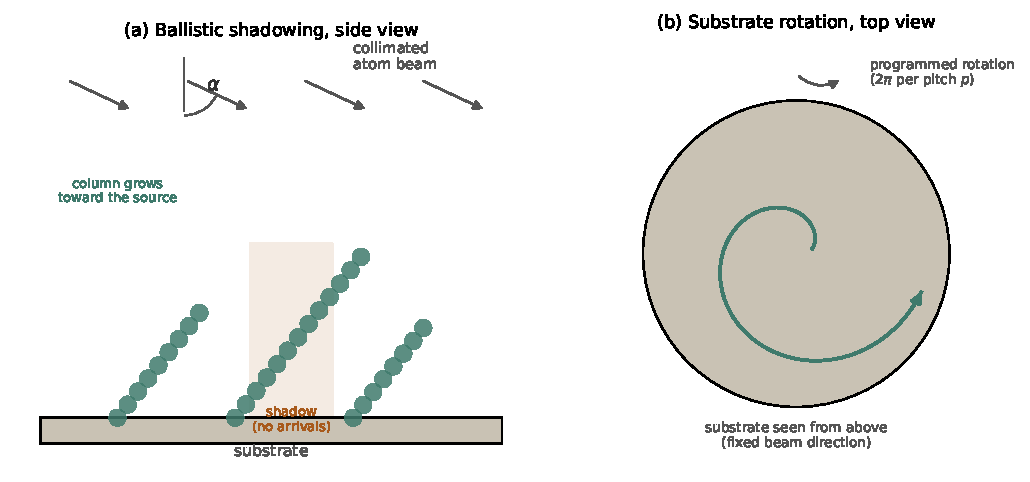
\includegraphics[width=0.85\linewidth]{deposition_schematic}
  \caption{%
    The two knobs an experimentalist turns on a GLAD chamber -- beam tilt
    $\dang$ and substrate rotation -- are exactly the two inputs to this
    simulator; everything else (columns, shadowing, voids) is an emergent
    consequence of these two settings plus first-contact sticking.
    Schematic of the ballistic deposition mechanism (conceptual diagram,
    not simulation output; compare Figure~\ref{fig:crosssection} for the
    simulator's actual output).
    (a) Side view: atoms arrive as a collimated beam at angle $\dang$ from
    the substrate normal and stick irreversibly on first contact, with no
    subsequent surface diffusion. A column that nucleates first casts a
    geometric shadow (shaded region) that suppresses further arrivals
    immediately behind it -- this is the entire origin of the void
    fraction trend in Section~\ref{sec:results_openness}.
    (b) Top view: the substrate rotates continuously during growth,
    tracing one full $2\pi$ turn per helical pitch $p$, which is what
    makes the resulting columns helical rather than straight.
  }
  \label{fig:deposition_schematic}
\end{figure}

Physically, the simulator asks a simple question: if atoms travel in
straight lines from the source and stop irreversibly the instant they
touch another atom or the substrate---i.e.\ if the only thing shaping the
film is geometric shadowing, with no atom motion after landing---how much
of the deposited volume ends up empty (void) rather than filled (solid),
and how does that depend on the deposition angle $\dang$ that an
experimentalist sets on the chamber? Simulations were performed with a
custom bead-sphere ballistic deposition code.  Atoms are launched from a collimated beam
incident at angle $\dang$ from the substrate normal.  Each atom follows
a straight-line (ballistic) trajectory and sticks irreversibly to the
first atom it contacts; no surface diffusion, relaxation, or
evaporation is included.  The film grows on a square substrate of
lateral size $L_x \times L_y = \SI{100}{nm} \times \SI{100}{nm}$ with
periodic (minimum-image) boundary conditions in the two in-plane
directions.
The model contains no material-specific physics: ``Cu'' enters only through
the hard-sphere atomic radius (i.e.\ a Cu-scale length), not through any
Cu-specific diffusion, sticking, or energetic parameter.  The simulator is
therefore a \emph{generic hard-sphere ballistic helical GLAD model
parameterised at a Cu atomic scale}, and the geometric outputs apply to any
material only insofar as its real morphology is shadowing-dominated; the
later substitution of tungsten optical constants (Section~\ref{ssec:nif_optical})
is an illustrative material substitution, not a calibrated W-film model.

\subsection{Helical substrate and parameter space}
\label{ssec:params}

Physically, this subsection reproduces in simulation the two knobs an
experimentalist actually turns during a helical GLAD run: the fixed
deposition angle $\dang$ (substrate tilt relative to the vapour beam) and
the programmed substrate rotation that traces out one helical turn per
pitch length $p$; the goal is to isolate how much of the resulting
morphology change is due to $\dang$ alone, holding the rotation program
and target film height fixed. A helical hard-sphere nanostructure template
is defined with target height
$h = \SI{300}{nm}$ and helical pitch $p = \SI{150}{nm}$ (two full
turns within the film).  The pitch is a controlled numerical reference
derived from the standard helix pitch relation using the vertical-growth-rate
convention; it is used here to isolate deposition-angle dependence and is
not presented as an experimentally calibrated Cu pitch. Pitch is routinely
varied in the GLAD literature to target specific structural and optical
outcomes rather than fixed by an underlying physical constant
\citep{park2009pitch}, and the value used here specifies the growth
condition studied on that same basis.
The void-fraction and deposited-atom-count dataset reported in
Section~\ref{sec:results_openness} comprises eight production
configurations, one realization each, at $\dang \in \{60, 65, 70, 75, 80,
85, 87, 89\}^{\circ}$; $\dang = 87^{\circ}$ is a planned addition to this
dataset and is reported as pending wherever it appears below. The
descriptor-space analyses of Sections~\ref{ssec:pca}
and~\ref{ssec:nif_methods} draw on an extended voxel-field dataset that
additionally includes repeated independently-seeded realizations at
$\dang = 80^{\circ}$ and $85^{\circ}$, as described in those sections.
A separate simulation at $\dang = 72^{\circ}$ was subsequently performed
exclusively as a prospective validation case for the \textsc{CorrNIF}
interpolation (Section~\ref{ssec:nif_prospective}); it was excluded from
CorrNIF training and from all main-dataset descriptive analyses.
The deposition angle $\dang$ is measured from the substrate normal, and the
helix is generated by programmed azimuthal rotation of the substrate during
growth (one $2\pi$ azimuthal turn per pitch length $p$).
Table~\ref{tab:params} collects the simulation and analysis parameters for
reproducibility; quantities not separately parameterised in this ballistic
model (beam angular divergence, arrival-position distribution beyond uniform
random azimuth, explicit nucleation/sticking rules) are defined by the
simulation code (available from the corresponding author) rather than by tunable inputs.

Before the quantitative characterisation that follows, Figure~\ref{fig:crosssection}
shows directly what the simulator produces: real voxelised cross-sections of a
simulated film, not a schematic. At $\dang=89^{\circ}$, the lateral (\textit{xy})
slice shows isolated, well-separated columns rather than a continuous film, and
the vertical (\textit{xz}) slice shows these columns as tilted streaks -- the
geometric shadowing signature that the tangent rule and the void-fraction trend
in Section~\ref{sec:results_openness} both quantify. At $\dang=60^{\circ}$, the same
lateral slice is nearly fully covered, consistent with the much lower void
fraction at this shallower angle.

\begin{figure}[htbp]
  \centering
  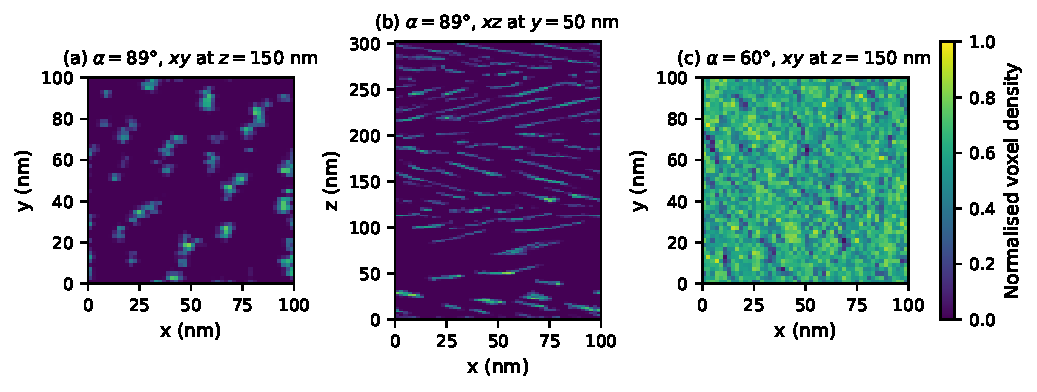
\includegraphics[width=0.95\linewidth]{morphology_crosssection}
  \caption{%
    Direct visual evidence of the shadowing mechanism that the rest of this
    paper characterises quantitatively: isolated, tilted columns at high
    $\dang$ versus a near-continuous film at low $\dang$.
    Voxelised density cross-sections of simulated Cu GLAD films
    ($h=\SI{300}{nm}$, pitch $=\SI{150}{nm}$, seed 1, \SI{2}{nm} voxels).
    (a) Lateral (\textit{xy}) slice at mid-height ($z=\SI{150}{nm}$),
    $\dang=89^{\circ}$: isolated columns, $8.2\%$ occupied.
    (b) Vertical (\textit{xz}) slice at $y=\SI{50}{nm}$, $\dang=89^{\circ}$:
    the same columns appear as tilted streaks, the direct signature of
    ballistic shadowing along the deposition direction.
    (c) Lateral slice at $\dang=60^{\circ}$ for comparison: $83.5\%$ occupied,
    a near-continuous film at this shallower angle.
    Despite occupying only $8.2\%$ of the volume at $\dang=89^{\circ}$, the
    column network remains fully percolated (largest connected fraction
    $=0.974$, i.e.\ essentially all deposited material belongs to one
    connected structure spanning the film).
  }
  \label{fig:crosssection}
\end{figure}

\begin{table}[htbp]
  \centering
  \caption{%
    Simulation and analysis parameters.  Quantities marked ``code'' are
    fixed by the ballistic simulator code rather than exposed as tunable
    inputs.}
  \label{tab:params}
  \begin{tabular}{p{0.36\linewidth}p{0.28\linewidth}p{0.27\linewidth}}
    \toprule
    Parameter & Value & Source/status \\
    \midrule
    \multicolumn{3}{l}{\emph{Geometry and domain}}\\
    Substrate lateral size $L_x\times L_y$ & $\SI{100}{nm}\times\SI{100}{nm}$ & prescribed in this work \\
    Lateral boundary conditions & periodic (minimum-image), XY & simulator setting \\
    Target film height $h$ & \SI{300}{nm} & prescribed in this work \\
    Final height range (8 runs) & \SI{300.00}{nm}--\SI{300.15}{nm} & simulation result, this work \\
    Helical pitch $p$ (turns) & \SI{150}{nm} (2 turns in $h$) & controlled numerical reference; not Cu-calibrated \\
    Deposition-angle convention & polar, from substrate normal & simulator convention \\
    Azimuthal rotation law & programmed, $2\pi$ per pitch length & derived from prescribed pitch \\
    \multicolumn{3}{l}{\emph{Ballistic deposition model}}\\
    Hard-sphere radius $R$ (diameter $2R$) & \SI{0.128}{nm} (\SI{0.256}{nm}) & Cu covalent (Cordero) radius \citep{cordero2008}; Section~\ref{ssec:sim_params} \\
    First-contact criterion & $2R$ physical contact & simulator rule \\
    Sticking probability & 1 (irreversible, first contact) & simulator rule \\
    Surface diffusion / re-emission / evap. & none / none / none & prescribed model scope \\
    Re-emission, angular divergence & none; collimated beam & prescribed model scope \\
    XY launch distribution & uniform random over the cell & simulator rule \\
    Initial seed layer & $10^{4}$ seed atoms & numerical setting, this work \\
    Nominal deposition rate & \SI{0.3}{nm/s} (dense-equiv.) & within the range reported for GLAD Cu/metal deposition \citep{jamnig2019} \\
    Substrate temperature & not active in the ballistic physics & not used by this model \\
    ``Cu'' material content & hard-sphere radius (a Cu-scale length) only & not a calibrated Cu model \\
    Deposited atoms per run (void-fraction dataset) & $4.5\times10^{6}$--$4.1\times10^{7}$ & simulation result, this work \\
    Stopping criterion & target height $h=\SI{300}{nm}$ reached & prescribed in this work \\
    Random seeds (RNG), void-fraction dataset & seed 0, one realization per angle & numerical setting, this work \\
    Random seeds (RNG), descriptor-space dataset & 1 per angle; 3 at $80^{\circ},85^{\circ}$ & numerical setting, this work (Sections~\ref{ssec:pca}, \ref{ssec:nif_methods}) \\
    \multicolumn{3}{l}{\emph{Voxelisation and correlation}}\\
    Voxel grid & $50\times50\times151$ (\SI{2}{nm} XY, \SI{2}{nm} Z) & numerical setting, this work \\
    Voxelisation kernel & Gaussian bead-centre histogram & analysis setting \\
    Kernel / density normalisation & max-normalised, $\rho_{\rm voxel}\in[0,1]$ & analysis setting \\
    Occupancy threshold & $\rho_{\rm voxel}>0.5$ & analysis setting \\
    Derotation interpolation & bilinear, periodic wrap & corrected analysis setting \\
    Correlation radial binning & integer-voxel shells & analysis setting \\
    Correlation radial range & $r\le 24$~vox $\approx L/2$ (trusted $\lesssim10$~vox $\approx\SI{20}{nm}$) & finite-domain analysis choice \\
    \multicolumn{3}{l}{\emph{Illustrative optical screening}}\\
    Optical wavelength $\lambda$ & $\approx\SI{500}{nm}$ & prescribed screening wavelength \\
    Column dielectric (illustrative, W) & $\varepsilon_{\rm W}=4.41+19.60i$ & Ref.~\cite{palik1985} \\
    Host dielectric & $\varepsilon_h=1$ (vacuum) & prescribed screening host \\
    Optical film thickness & \SI{300}{nm} & same prescribed film height \\
    \bottomrule
  \end{tabular}
\end{table}
\subsection{Simulation parameters}
\label{ssec:sim_params}

Table~\ref{tab:sim_params_justified} collects the physical basis for the
parameters in Table~\ref{tab:params} that carry an independent literature
or first-principles justification, as distinct from the numerical and
analysis settings chosen for tractability. Each value is fixed
independently of the deposition angle $\dang$ and held constant across
the campaign described above.

\begin{table}[htbp]
  \centering
  \caption{%
    Simulation parameters and their physical basis.
  }
  \label{tab:sim_params_justified}
  \begin{tabular}{lll}
    \toprule
    \parbox{0.30\linewidth}{Parameter} & \parbox{0.22\linewidth}{Value} & \parbox{0.40\linewidth}{Basis / source} \\
    \midrule
    \multicolumn{3}{l}{\emph{Atomic and lattice scale}}\\
    \parbox{0.30\linewidth}{Cu atomic (covalent) radius $r$} & \parbox{0.22\linewidth}{\SI{0.128}{nm}} & \parbox{0.40\linewidth}{Cordero covalent radius \citep{cordero2008}} \\
    \parbox{0.30\linewidth}{Hard-sphere collision diameter $2r$} & \parbox{0.22\linewidth}{\SI{0.256}{nm}} & \parbox{0.40\linewidth}{derived directly from $r$} \\
    \parbox{0.30\linewidth}{Substrate seed spacing} & \parbox{0.22\linewidth}{\SI{0.256}{nm}} & \parbox{0.40\linewidth}{matches the Cu FCC nearest-neighbour distance $a/\sqrt{2}=\SI{0.2556}{nm}$ for lattice constant $a=\SI{3.615}{\angstrom}$ \citep{straumanis1969}; agreement between the covalent-radius and lattice-geometry routes is within $0.16\%$} \\
    \multicolumn{3}{l}{\emph{Growth kinetics}}\\
    \parbox{0.30\linewidth}{Deposition rate} & \parbox{0.22\linewidth}{\SI{0.3}{nm/s}} & \parbox{0.40\linewidth}{within the range reported for GLAD Cu/metal deposition, $\approx\SI{0.2}{}$--\SI{0.5}{nm/s} \citep{jamnig2019}} \\
    \parbox{0.30\linewidth}{Sticking coefficient (baseline)} & \parbox{0.22\linewidth}{$1.0$} & \parbox{0.40\linewidth}{idealised ballistic assumption; sensitivity tested at $s=0.2,0.5,1.0$ with no topology dependence found over this range (Section~\ref{ssec:connectivity_robustness})} \\
    \parbox{0.30\linewidth}{Diffusion activation energy $E_a$ (diffusion-enabled runs, Section~\ref{ssec:diffusion_comparison})} & \parbox{0.22\linewidth}{\SI{0.49}{eV}--\SI{0.5106}{eV}} & \parbox{0.40\linewidth}{the Boisvert--Lewis isolated-adatom value \citep{boisvert1997cu} and the Jamnig et al.\ Cu-on-amorphous-carbon value \citep{jamnig2019} used directly in the diffusion runs agree with an independent nudged-elastic-band calculation on the Mishin et al.\ Cu embedded-atom potential \citep{mishin2001cu} and with the Mehl et al.\ Cu(001) hopping-barrier fit \citep{mehl1999} to within $0.02$--$0.03$~eV} \\
    \multicolumn{3}{l}{\emph{Deposition geometry}}\\
    \parbox{0.30\linewidth}{Domain width/depth $L_x\times L_y$} & \parbox{0.22\linewidth}{$\SI{100}{}\times\SI{100}{nm}$} & \parbox{0.40\linewidth}{computational domain size chosen for numerical tractability under GPU memory constraints; box-size dependence characterised separately (Appendix~\ref{app:boxconv})} \\
    \parbox{0.30\linewidth}{Helical pitch $p$} & \parbox{0.22\linewidth}{\SI{150}{nm}} & \parbox{0.40\linewidth}{geometric parameter defining this study's helical growth condition (Section~\ref{ssec:params})} \\
    \bottomrule
  \end{tabular}
\end{table}

The atomic and lattice-scale parameters converge from two independent
routes: the Cordero covalent radius of Cu \citep{cordero2008} and the FCC
lattice geometry implied by the Cu lattice constant
$a=\SI{3.615}{\angstrom}$ \citep{straumanis1969} agree to within $0.16\%$
on the same underlying Cu--Cu contact length scale, and this length scale
sets both the hard-sphere collision diameter and the substrate seed
spacing used throughout. The diffusion parameters governing the
diffusion-enabled runs (Section~\ref{ssec:diffusion_comparison}) are
similarly cross-validated: an independent nudged-elastic-band calculation
on the Mishin et al.\ Cu embedded-atom potential \citep{mishin2001cu}
agrees with the two literature values used directly in this work
\citep{boisvert1997cu,jamnig2019} and with a further independent Cu(001)
hopping-barrier fit \citep{mehl1999} to within $0.02$--$0.03$~eV.

The helical pitch, $p=\SI{150}{nm}$, is the geometric parameter that
defines this study's helical growth condition. Pitch is routinely varied
in the GLAD literature to target specific structural and optical outcomes
rather than fixed by an underlying physical constant
\citep{park2009pitch}; the value used here specifies the growth
condition studied and is reported as such, without implying that a single
pitch value is independently prescribed by theory.


\subsection{Void-fraction definition}
\label{ssec:vf}

Physically, this quantity is the porosity-like measure of the film: the
fraction of the deposited volume that is empty space between column atoms
rather than solid material, computed geometrically from the known
hard-sphere size and count of the deposited atoms rather than from an
imaging or scattering measurement.
The bead-sphere void fraction is defined as:
\begin{equation}
  \bsP = 1 - \frac{N V_b}{L_x \, L_y \, z_{\max}},
  \qquad
  V_b = \tfrac{4}{3}\pi R^3,
  \label{eq:bead_sphere}
\end{equation}
where $N$ is the number of deposited atoms, $R$ is the atom radius,
and $z_{\max}$ is the height of the topmost atom.  This quantity
directly corresponds to the open volume in the idealised hard-sphere
packing and is logged by the simulator at the end of each simulation run.
It differs from the voxel-mean quantity $1 - \langle\rho_{\rm voxel}\rangle$
used for density-field analyses (Sections~\ref{sec:results_zprofile}
and~\ref{sec:results_pca}).

\subsection{Voxel density field}
\label{ssec:voxel}

Physically, this step turns the raw list of atom positions into something
directly comparable to a depth-resolved microstructure map, analogous to a
reconstructed FIB-SEM or nano-CT tomogram of a real film, so that how dense
or open the structure is at a given depth and lateral position can be
tracked separately from the single, film-averaged void fraction of
Section~\ref{ssec:vf}.
For depth-resolved and PCA analyses, atom positions are projected onto a
$50 \times 50 \times 151$ voxel grid ($\SI{2}{nm}$ XY resolution,
$\SI{2}{nm}$ Z resolution, spanning the
$\SI{100}{nm}\times\SI{100}{nm}\times\SI{300}{nm}$ cell)
using a Gaussian bead-centre kernel.  The resulting
normalised density field $\rho_{\rm voxel}(\mathbf{r}) \in [0,1]$
encodes the local atom-sphere overlap fraction, with the continuous
three-dimensional material distribution sampled on a regular spatial grid
as in the tomographic analogy above.
Each production run's checkpoint was verified before use: deposited atom
count matches the stored position array, final height falls within
\SI{0.15}{nm} of the \SI{300}{nm} target, and no invalid (NaN) position
entries are present. The $\dang = 60^{\circ}$ value used in the
openness-trend curve, $\bsP = 94.2\%$, is drawn from a checkpoint passing
all three checks.

\subsection{Morphological descriptors and PCA}
\label{ssec:pca}

Physically, a single voxel field contains far more information than an
experimentalist can compare across many deposition angles at a glance; the
goal here is to compress each film down to a handful of numbers that
capture how open it is, how directionally lopsided its columns are, and
whether the columns broaden or narrow with depth, and then to check
whether deposition angle alone organises these numbers into a simple,
low-dimensional trend.
This descriptor-space dataset comprises twelve voxel fields from the
extended, repeated-seed campaign described in Table~\ref{tab:params}
(eight angles plus two additional independently-seeded realizations each
at $80^{\circ}$ and $85^{\circ}$); one $\dang = 60^{\circ}$ voxel field had
a corrupted checkpoint (an active-slab resume duplication artefact giving a
physically impossible atom count) and is excluded, leaving eleven valid
voxel files. For each of these we use three non-redundant
descriptors:
(i)~openness proxy $1 - \langle\rho_{\rm voxel}\rangle$;
(ii)~XY anisotropy ratio (ratio of power along orthogonal in-plane axes);
(iii)~apparent width-gradient proxy (linear fit to column-width growth with
depth; used only as a descriptive feature, not interpreted as a
physical fanning exponent).
We deliberately exclude the mean filling fraction
$\langle\rho_{\rm voxel}\rangle$, which is exactly complementary to the
openness proxy ($\text{openness} = 1 - \langle\rho_{\rm voxel}\rangle$):
including both perfectly collinear measures double-counts the density axis
and artificially inflates the variance attributed to it on the leading
component.
Features are standardised before PCA; principal components are computed
via SVD, and variance fractions and loadings are reported.
The eleven observations include repeated seeds at $80^{\circ}$ and
$85^{\circ}$, which we keep as individual points (rather than averaging) so
that the seed-to-seed scatter is visible.
The result is therefore an exploratory descriptor-space summary, not a
demonstration of a general morphology manifold.

\subsection{Statistical morphology pipeline}
\label{ssec:nif_methods}

\subsubsection*{Corotating-frame pair correlation}

Physically, this descriptor asks how likely a column is to be found at a
given lateral distance from another column, once the steady rotation of
the substrate has been numerically ``undone'' so that a static column
arrangement, rather than a rotating helix, is being compared from film to
film; it is the real-space analogue of the column-spacing information
that a scattering experiment (SAXS/GISAXS) would extract from the
diffraction pattern of the same film.
The corotating-frame correlation starts from the binary occupancy field
$I(\mathbf{r}) = [\rho_{\rm voxel} > 0.5]$, from which the filling fraction
$f = \langle I \rangle$ is taken.
Each $z$-slice $I(\cdot,\cdot,k)$ is then derotated by the local helix
phase $\phi(k) = 2\pi k/p_{\rm vox}$, where $p_{\rm vox} = p/\Delta z$
is the pitch in voxels, using bilinear interpolation to avoid the
pixel-level jitter that nearest-neighbour resampling accumulates over
the 151 $z$-slices.  Because the domain is periodic, the bilinear
resampling uses periodic (wrap) source coordinates rather than
edge-clamped coordinates; the clamped variant violates per-slice mass
conservation by up to $10\%$ near the boundary and is therefore replaced
here.  Switching from the edge-clamped to the periodic-wrap derotation
perturbs $h_g$ by a mean absolute difference of $0.007$ over the full curve
($0.015$ at short range, where the steep near-origin drop amplifies small
horizontal shifts; maximum pointwise $0.035$).  This is comparable to the
intrinsic seed-to-seed scatter ($\approx0.008$, below) and leaves the
angle ordering and every qualitative conclusion unchanged
(validation tests included with the analysis code).
Bilinear derotation maps the binary slice to a \emph{continuous} occupancy
field $J\in[0,1]$, for which the binary identity $\langle J^2\rangle=\langle
J\rangle$ no longer holds; we therefore normalise by the empirical
zero-lag (continuous-covariance) variance rather than by the binary
value $1/f$ (Eqs.~\ref{eq:pair_corr}--\ref{eq:hg_norm}).
The circular autocorrelation $C(r)=\langle J(\mathbf{x})J(\mathbf{x}+r)\rangle$
is obtained by FFT, radially averaged, and the result is averaged over all
$z$-slices to yield the ensemble-mean corotating-frame curve
$\langle h_g(r;\dang)\rangle_z$.
This is computed for the seven single-seed configurations
$\dang \in \{65, 70, 75, 80, 85, 87, 89\}^{\circ}$.
The lateral domain is $\SI{100}{nm}$ with periodic boundaries, and the radial
average is taken to $r_{\max}\approx 24$~voxels ($\approx\SI{48}{nm}$), i.e.\
close to half the box width $L/2$.  Under the periodic (minimum-image)
convention the correlation near $r\to L/2$ is constrained by the finite
domain, so the curves are informative mainly at short range
($r \lesssim 10$~voxels $\approx\SI{20}{nm}$, the regime that dominates the
descriptor and the emulator targets) and the long-range tail should be read
with caution.  A box-size convergence study (e.g.\ $100$, $150$, $200$~nm at
representative angles) would be required to confirm that the short-range
correlation is free of finite-size or periodic artefacts; this requires new
simulations and is left as future work. (A related but distinct check --
bulk atom-density convergence with box size at fixed pitch, not the
correlation function itself -- was performed and found NOT converged at
$L=\SI{100}{nm}$; see the box-size limitation in Section~\ref{ssec:limits}.)

\subsubsection*{CorrNIF architecture and training}

\textsc{CorrNIF} is a compact parametric emulator that maps deposition
angle $\dang$ and radial distance $r$ to the predicted pair-correlation
value $h_g(r;\dang)$ at any combination of these two inputs---analogous
to a parametric dispersion model that evaluates a refractive-index
spectrum at any wavelength and filling fraction without re-running a
full electromagnetic simulation.

A compact neural implicit field (\textsc{CorrNIF}) maps
$(\dang_{\rm norm}, r_{\rm norm}) \to h_g(r;\dang)$, where
$\dang_{\rm norm} = (\dang - 74.5^{\circ})/14.5^{\circ}$ and
$r_{\rm norm} = r/r_{\rm max}$.
The radial coordinate is encoded via $n_{\rm freq} = 12$ random Fourier
features \citep{tancik2020}:
$\mathbf{h}_0 = [\sin(2\pi\mathbf{B}r),\cos(2\pi\mathbf{B}r)]$,
$\mathbf{B} \sim \mathcal{N}(0,\sigma_r^2)$, $\sigma_r = 2$.
Three fully connected hidden layers (width~64, SiLU activation) receive
angle conditioning (feature-wise linear modulation, FiLM) from $\dang$:
$\mathbf{h}_{i+1} =
  \mathrm{SiLU}\!\bigl[(1+0.1\gamma_i)\mathbf{W}_i\mathbf{h}_i
  + 0.1\beta_i\bigr]$,
where $(\gamma_i,\beta_i)$ are produced by an $\dang$-conditioned
two-layer MLP (width~32, ReLU).
Figure~\ref{fig:corrnif_arch} summarises this architecture.

\begin{figure}[htbp]
  \centering
  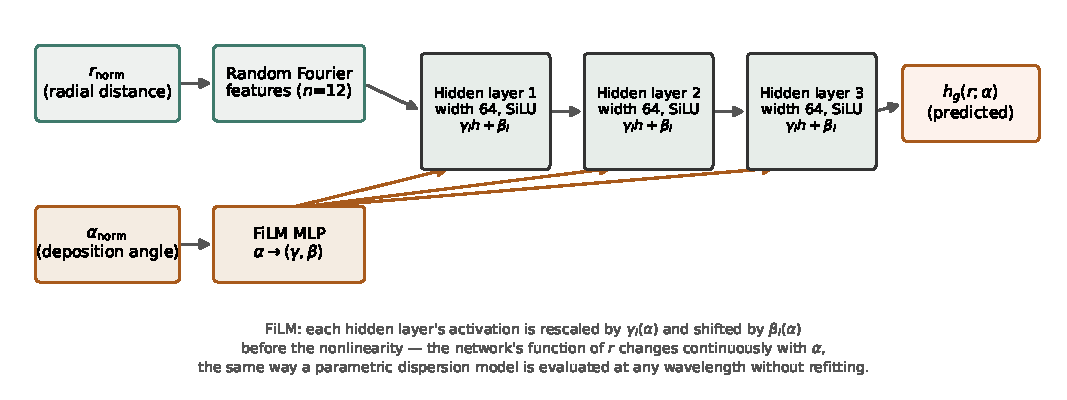
\includegraphics[width=0.95\linewidth]{corrnif_architecture}
  \caption{%
    The angle conditioning does not add a third input alongside $r$; it
    reshapes the network's response to $r$ at every layer, which is why a
    single trained model can be evaluated smoothly at angles it never saw
    during training (Section~\ref{ssec:nif_prospective}).
    Schematic of the \textsc{CorrNIF} architecture (conceptual diagram).
    The radial coordinate $r$ is Fourier-encoded and passed through three
    FiLM-conditioned hidden layers; the deposition angle $\dang$ does not
    enter as a third raw input but instead rescales ($\gamma_i$) and
    shifts ($\beta_i$) each layer's activation via a small side network,
    analogous to how a parametric dispersion model is evaluated at any
    wavelength without being refitted at that wavelength.
  }
  \label{fig:corrnif_arch}
\end{figure}

Training uses the Adam optimiser (learning rate $10^{-3}$,
1000 epochs, batch size~512, MSE loss on $h_g$).
For the corrected analysis reported here, \textsc{CorrNIF} was retrained
from scratch on the periodic-wrap, continuous-covariance target; ten
independent neural initialisations were run for each validation fold and
for the prospective $72^{\circ}$ case.
Generalisation is evaluated by a seven-fold leave-one-angle-out (LOOA)
protocol: in each fold, \textsc{CorrNIF} is trained on six deposition
angles and used to predict $h_g(r;\dang_{\rm held})$ without any
adaptation on the held-out angle---analogous to fitting an optical
dispersion model to spectra measured at six incidence angles and
evaluating its prediction at a seventh, held-out angle.

\subsubsection*{Maxwell-Garnett effective-medium model}

Physically, this step asks what optical anisotropy a film with the
simulated column filling fraction $f(\dang)$ would show \emph{if} its
electromagnetic response could be approximated by smoothly averaging the
column and void dielectric properties together, rather than by resolving
the actual column geometry wave-optically---a standard first estimate of
form birefringence, used here as a scoping tool rather than a precision
prediction.
Effective optical properties are derived from the Maxwell-Garnett (MG)
effective-medium approximation for \emph{aligned} cylindrical inclusions in
a host medium \citep{maxwell1904} (Figure~\ref{fig:mg_concept}), a special
case of the broader family of
mixing formulas surveyed by \citet{sihvola1999mixing} and related to the
symmetric effective-medium approximation of \citet{bruggeman1935};

\begin{figure}[htbp]
  \centering
  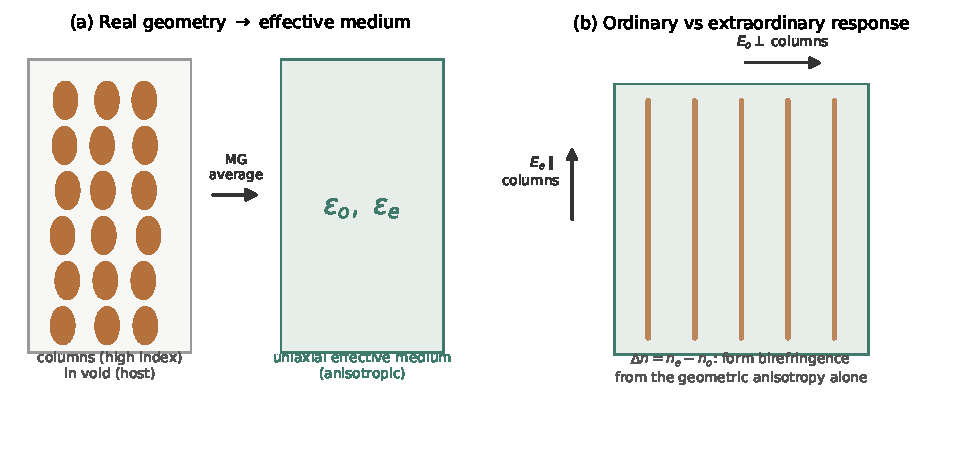
\includegraphics[width=0.95\linewidth]{maxwell_garnett_concept}
  \caption{%
    The birefringence reported below is not an extra material property
    being added to the model; it falls directly out of averaging an
    already-anisotropic column geometry into a single effective medium.
    Conceptual illustration of the Maxwell-Garnett effective-medium
    approximation (not simulation output).
    (a) Aligned high-index cylindrical inclusions (columns) embedded in a
    low-index host (void) are replaced by a single uniaxial effective
    medium with two principal dielectric constants, $\varepsilon_o$ and
    $\varepsilon_e$.
    (b) The two principal optical axes: the extraordinary axis
    $E_e$ lies parallel to the columns, the ordinary axis $E_o$
    perpendicular to them. Form birefringence $\Delta n = n_e - n_o$
    arises purely from this geometric anisotropy, before any intrinsic
    material birefringence is considered.
  }
  \label{fig:mg_concept}
\end{figure}
empirical extensions of this approach specifically fitted to the measured
principal refractive indices of obliquely deposited oxide sculptured thin
films (Ta$_2$O$_5$, TiO$_2$, ZrO$_2$) are given by
\citet{hodgkinson1998empirical}, building on the birefringent-thin-film
formalism of \citet{hodgkinson1997birefringent}.
This describes a uniaxial medium with the optic axis along the column
direction; it is a local, aligned-column approximation and does \emph{not}
capture the rotating optic axis, circular birefringence, or circular
dichroism of a true helical (chiral) film, nor pitch-scale resonances or
spatial dispersion.  The quasi-static homogenisation underlying MG requires
the structural period to be small compared with the wavelength; here the
helical pitch $p = \SI{150}{nm}$ and $\lambda \approx \SI{500}{nm}$ give
$p/\lambda \approx 0.30$, which is not deep in the quasi-static limit, so
the calculation should be read as an order-of-magnitude screening estimate
of the \emph{local} form birefringence of an aligned columnar array rather
than as the full optical response of the helical architecture.
As a sensor-design hypothesis-generation illustration only, column dielectric
functions are taken from tungsten ($\varepsilon_{\rm W} = 4.41 + 19.60i$ at
$\lambda \approx \SI{500}{nm}$, corresponding to optical constants
$n = 3.5$, $k = 2.8$ \citep{palik1985}) in a vacuum host
($\varepsilon_h = 1$).  Both the ordinary ($\varepsilon_o$, transverse
polarisation) and extraordinary ($\varepsilon_e$, longitudinal, Wiener
parallel limit) dielectric functions (Eqs.~\ref{eq:mg_transverse}
and~\ref{eq:mg_parallel}) are evaluated as complex quantities, and the
effective indices are obtained as $N=\sqrt{\varepsilon}$ on the passive
(positive-imaginary) branch, so that both refractive index $n$ and
extinction $k$ are retained for each polarisation.
The filling fraction $f(\dang)$ is \emph{not} a unique material-independent
quantity: the ballistic geometry yields two distinct measures (the
bead-sphere solid fraction $1-\bsP$ and the thresholded voxel occupancy
$f_{\rho>0.5}$) that differ by up to a factor of four
(Section~\ref{ssec:nif_optical}).  Real GLAD morphology is moreover
material-dependent through surface diffusion, sticking, re-emission,
homologous temperature, deposition rate, and pressure; the substitution of
W (or Mo, Co) optical constants into the Cu-scale geometry is therefore an
illustrative material substitution, not a prediction of a realisable W
film, and any quantitative transfer would require material-specific
calibration.

% ============================================================
\section{Results}
\label{sec:results}

\subsection{Bead-sphere void fraction}
\label{sec:results_openness}

This subsection addresses the void-fraction-trend half of \textbf{Q1} (the
comparison against published optical void fractions, the other half of
Q1, follows in Section~\ref{sec:results_lit}).
Figure~\ref{fig:openness} shows $\bsP$ as a function of deposition angle
for the eight main configurations ($\dang = 87^{\circ}$ pending; seven
angles shown). The void fraction increases monotonically from
$\bsP = \SI{94.2}{\%}$ at $\dang = 60^{\circ}$ to $\bsP = \SI{99.4}{\%}$ at
$\dang = 89^{\circ}$, consistent with the expected shadowing-enhancement at
high obliquity. Table~\ref{tab:repro} reports the void fraction and
deposited-atom count at each angle from its single production realization
(seed 0); with one realization per angle, run-to-run reproducibility is
not separately characterised in this revision.

\begin{figure}[htbp]
  \centering
  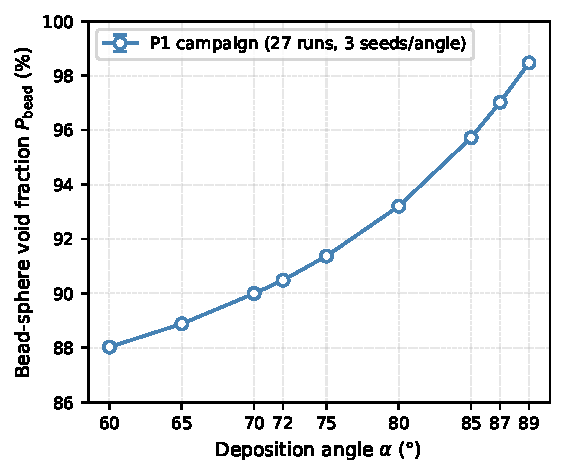
\includegraphics[width=0.78\linewidth]{levelA_openness_trend}
  \caption{%
    Steeper deposition angles produce systematically more open (porous)
    films.
    Bead-sphere void fraction $\bsP$ (Eq.~\ref{eq:bead_sphere}) as a
    function of deposition angle, one production realization (seed 0) per
    angle, for the main campaign ($\dang \in \{60, 65, 70, 75, 80, 85, 87,
    89\}^{\circ}$; $h = \SI{300}{nm}$, pitch $= \SI{150}{nm}$;
    $\dang = 87^{\circ}$ pending).
    The void fraction increases monotonically with $\dang$ over the seven
    angles completed to date, reaching $99.4\%$ at $\dang = 89^{\circ}$;
    per-angle values are given in Table~\ref{tab:repro}.
  }
  \label{fig:openness}
\end{figure}

\begin{table}[htbp]
  \centering
  \caption{%
    Bead-sphere void fraction $\bsP$ and deposited atom count $N$ at each
    deposition angle, single production realization (seed 0) per angle.
    $\rho_A$: deposited-atom areal density ($N$ per unit substrate area).
  }
  \label{tab:repro}
  \begin{tabular}{lccc}
    \toprule
    $\dang$ ($^{\circ}$) & $N$ (atoms) & $\bsP$ (\%) & $\rho_A$ (\si{nm^{-2}}) \\
    \midrule
    60 & $4.120\times10^{7}$ & 94.2 & 4120 \\
    65 & $3.804\times10^{7}$ & 94.7 & 3804 \\
    70 & $3.443\times10^{7}$ & 95.2 & 3443 \\
    75 & $2.960\times10^{7}$ & 95.9 & 2960 \\
    80 & $2.335\times10^{7}$ & 96.7 & 2335 \\
    85 & $1.468\times10^{7}$ & 98.0 & 1468 \\
    87 & \multicolumn{3}{c}{pending} \\
    89 & $4.540\times10^{6}$ & 99.4 & 454 \\
    \bottomrule
  \end{tabular}
\end{table}

\subsection{Depth-resolved void-fraction profiles}
\label{sec:results_zprofile}

This subsection addresses the depth-variation part of \textbf{Q2}.
Figure~\ref{fig:zprofile} shows the layer-wise void fraction
$1 - \bar{\rho}_z(z)$ (mean over the $50 \times 50$ XY grid at each
Z-slice) for all eleven valid configurations.

\begin{figure}[htbp]
  \centering
  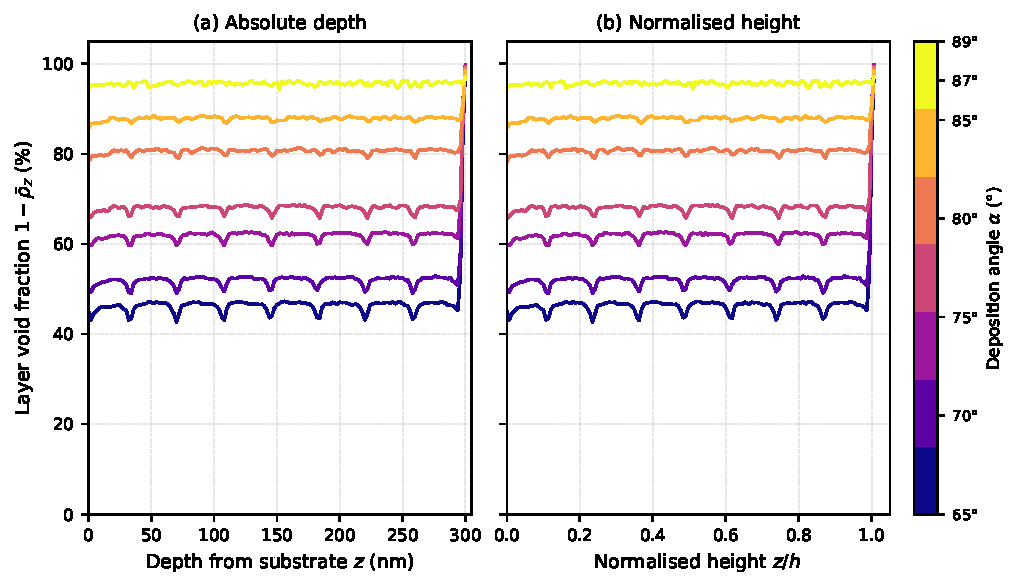
\includegraphics[width=\linewidth]{levelA_zprofile}
  \caption{%
    Every film has a denser layer near the substrate before opening up
    into the angle-dependent shadowing regime that dominates the bulk of
    the growth.
    Depth-resolved void fraction $1 - \bar{\rho}_z$ as a function of
    (a)~absolute depth from substrate ($z$) and (b)~normalised film height
    ($z/h$), for eleven helical Cu GLAD configurations spanning
    $\dang = 65^{\circ}$--$89^{\circ}$ (seed 0 for each angle;
    $\dang = 60^{\circ}$ excluded due to a voxelisation artefact at this angle).
    Curves are colour-coded by $\dang$ (plasma colourmap, $65^{\circ}$ = violet, $89^{\circ}$ = yellow).
    The quantity $1 - \bar{\rho}_z$ is the smeared-kernel void fraction
    averaged over the $100 \times 100$~nm$^2$ substrate plane at each depth slice,
    which differs from the global bead-sphere $\bsP$.
    All curves show a dense substrate layer ($z < 30$~nm) transitioning
    to a shadowing-dominated bulk regime.
  }
  \label{fig:zprofile}
\end{figure}

Three features are evident:
\begin{enumerate}
  \item \textit{Dense substrate layer.}  All configurations show a lower
    void fraction near the substrate ($z < \SI{30}{nm}$), reflecting the
    initial random-accumulation regime before columnar shadowing develops.
    This layer is thinner and less dense at higher $\dang$.

  \item \textit{Monotonic mid-film void fraction.}  The bulk columnar
    region (approximately $z = \SI{50}{nm}$--$h_{\rm top}$) shows a
    void fraction that increases with $\dang$, consistent with stronger
    shadowing.  At $\dang = 65^{\circ}$ the mid-film layer void fraction is
    approximately \SI{57}{\%}, whereas at $\dang = 89^{\circ}$ it approaches
    \SI{95}{\%}.

  \item \textit{Normalised-height convergence.}  When height is
    normalised by film top $z/h$ (panel~b), the mid-film profiles
    collapse more closely.  Because all films share essentially the same
    target height ($h \approx \SI{300}{nm}$), this normalisation cannot
    separate a growth-kinetics origin from an absolute-height origin; a
    height series at fixed $\dang$ (available in the levelB dataset but not
    analysed here) would be required to attribute the collapse to growth
    kinetics, and we report it only as an observed collapse.
    The profiles also show low-amplitude oscillations with depth; these are
    consistent with the helical rotation period and the finite voxel
    slice spacing and are not interpreted as a distinct physical growth
    modulation pending a dedicated sampling-convergence check.
\end{enumerate}

These depth gradients are relevant to optical and sensor properties, which
depend on the local void-fraction profile rather than the bulk average,
although a quantitative optical use would require the convergence checks
noted above.

\subsection{Morphology latent space}
\label{sec:results_pca}

This subsection addresses the low-dimensional-summary part of
\textbf{Q2}.
Figure~\ref{fig:pca} shows the PCA of the three non-redundant
morphological descriptors extracted from the eleven valid voxel fields.

\begin{figure}[htbp]
  \centering
  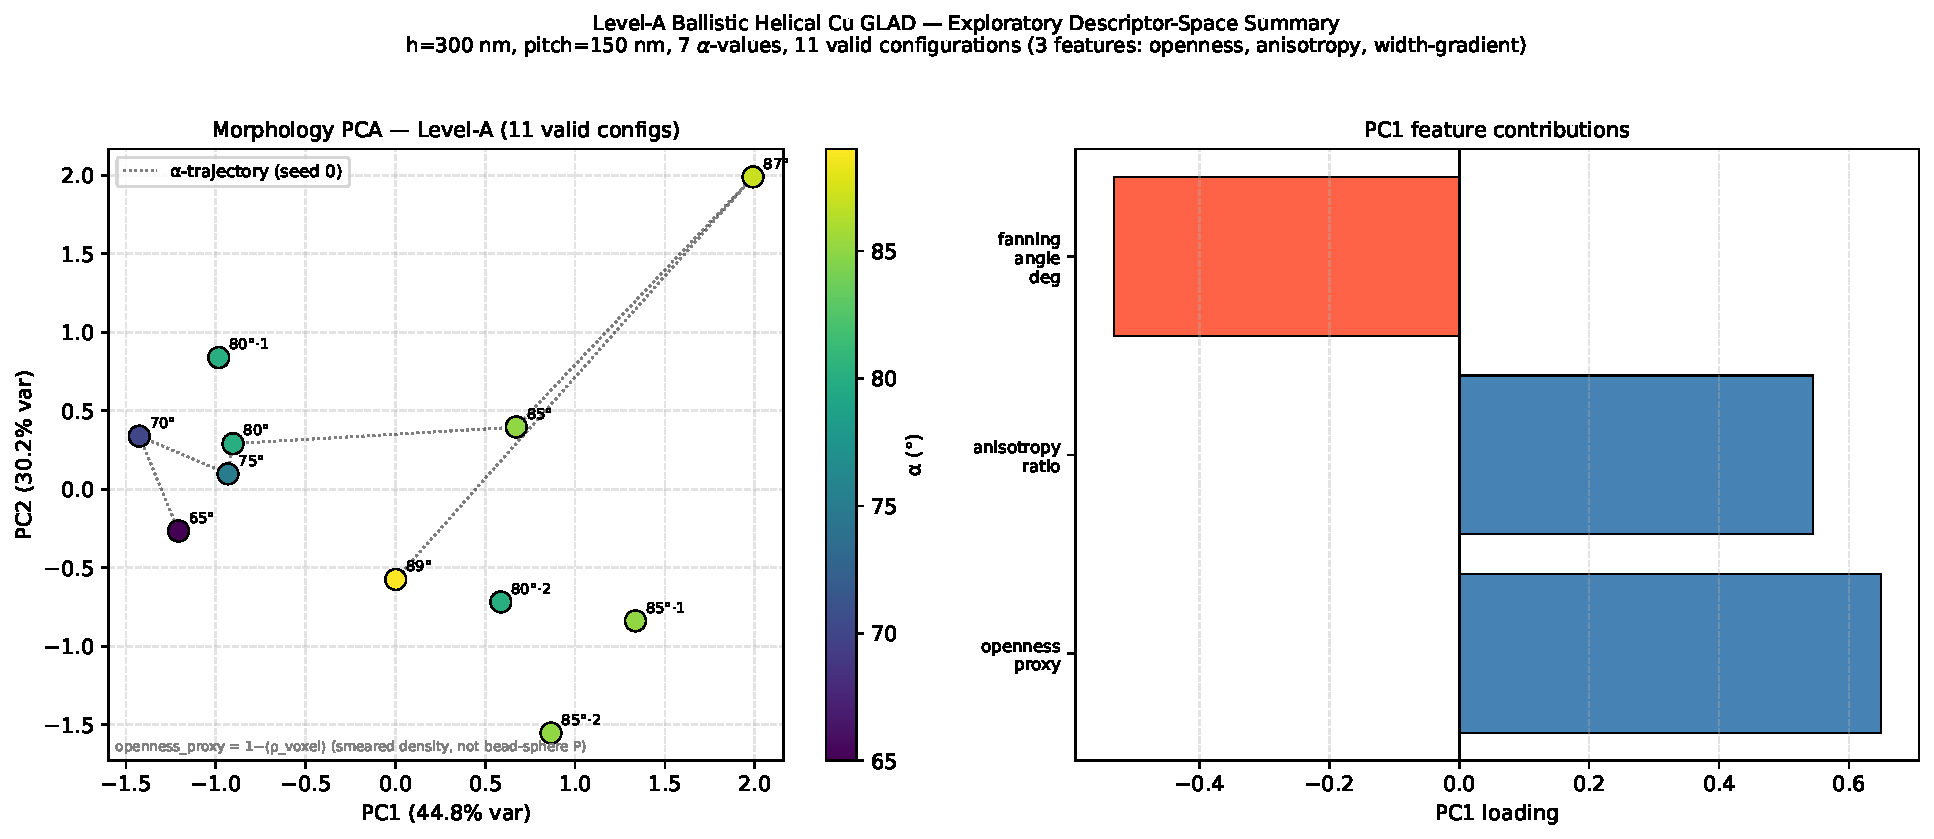
\includegraphics[width=\linewidth]{morphology_pca_space_levelA}
  \caption{%
    Deposition angle is the dominant organising variable in this
    three-descriptor morphology space, but repeated seeds at the same
    angle still scatter visibly, showing that only the bulk density trend,
    not the full morphology, is tightly reproducible.
    (a)~Principal component analysis (PCA) of three non-redundant
    morphological descriptors
    (openness $1-\langle\rho\rangle$, anisotropy ratio, apparent
    width-gradient proxy) for the eleven valid ballistic helical Cu GLAD
    voxel fields ($\dang = 60^{\circ}$ excluded due to a voxelisation
    artefact; the mean filling fraction is omitted as it is exactly
    complementary to openness).
    Points are colour-coded by deposition angle $\dang$; the dotted line
    connects the seed-0 points in order of increasing $\dang$, and the three
    seeds at $80^{\circ}$/$85^{\circ}$ appear as separate points to show the
    seed-to-seed scatter.
    The first two principal components capture $44.8 + 30.2 = 75\%$ of the
    descriptor variance in this exploratory three-feature summary (with three
    features the per-component null expectation is $33\%$, so PC1 is only
    moderately dominant).
    (b)~PC1 feature loadings: all three descriptors contribute comparably
    (openness $0.65$, anisotropy $0.54$, width-gradient $-0.53$), so PC1 is a
    blend rather than a single-descriptor axis.
  }
  \label{fig:pca}
\end{figure}

With the redundant filling fraction removed, the first two principal
components account for $44.8 + 30.2 = 75.0\%$ of the descriptor variance.
PC1 is now a balanced blend of all three descriptors
(loadings: openness $0.65$, anisotropy $0.54$, width-gradient $-0.53$)
rather than being dominated by the density measures, and PC2 is carried
mainly by anisotropy and the width-gradient ($-0.69$ and $-0.72$, openness
$\approx 0$).
The points show a broad shift toward larger PC1 as $\dang$ increases, but
the trajectory is not a clean monotonic locus: the three seeds at
$80^{\circ}$ and $85^{\circ}$ are visibly scattered in the PC1--PC2 plane.
Within this extended, repeated-seed dataset, the bulk density (openness)
is reproducible to sub-percent level across the three seeds at
$80^{\circ}$ and $85^{\circ}$, while the higher-order descriptors
(anisotropy, width gradient) carry visibly more run-to-run variability.
Within this fixed-height, fixed-pitch sweep, deposition angle is the
dominant \emph{controlled} source of descriptor variation, but---given only
eleven observations and three features, several of them repeated seeds---we
read this as an exploratory summary rather than evidence of a smooth
low-dimensional morphology manifold.

\subsection{Comparison with literature void fractions}
\label{sec:results_lit}

This subsection addresses the second half of \textbf{Q1}: the quantitative
comparison against published optical void fractions.
Figure~\ref{fig:lit} compares the ballistic bead-sphere void-fraction
curve with published optical void fractions for GLAD metal films at
$\dang = 85^{\circ}$ from Fischer \& Schubert (2013).

\begin{figure}[htbp]
  \centering
  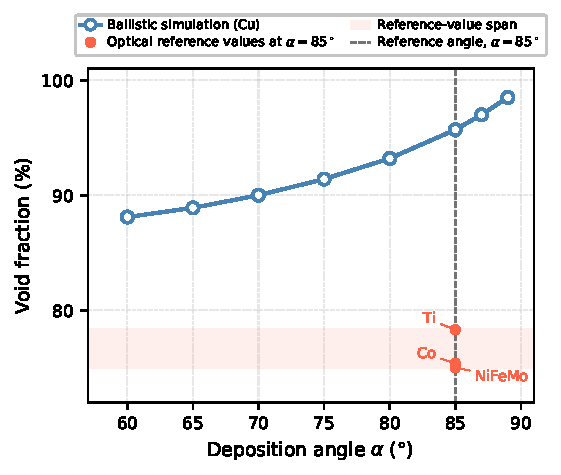
\includegraphics[width=0.82\linewidth]{levelA_vs_literature_comparison}
  \caption{%
    The purely geometric ballistic model is systematically more open than
    real deposited GLAD metal films, confirming that surface diffusion and
    measurement-convention differences (not captured by this model) matter
    quantitatively.
    Comparison of bead-sphere void fraction $\bsP$ (ballistic Cu GLAD
    simulation, blue curve) with published optical void fractions for
    GLAD metal films (Co: $75.4\%$; Ti: $78.3\%$; NiFeMo: $75.0\%$)
    at $\dang = 85^{\circ}$ measured by the anisotropic Bruggeman
    effective-medium approximation (ABEMA method; Fischer \& Schubert
    2013 \citep{fischerscubert2013}).
    Red points with error bars: individual published values;
    shaded band: literature range.
    The ballistic simulation overestimates the published median by
    $+23.0$~percentage points at $\dang = 85^{\circ}$.
    The three contributing sources of mismatch (absence of surface
    diffusion, measurement-convention difference, and material difference)
    are discussed in Section~\ref{ssec:limits}.
  }
  \label{fig:lit}
\end{figure}

At $\dang = 85^{\circ}$, the ballistic simulation yields $\bsP = 98.0\%$,
while the optical void fractions of GLAD metal films
(Co: $75.38 \pm 0.01\%$; Ti: $78.30 \pm 0.04\%$;
NiFeMo: $75.0 \pm 0.1\%$) cluster around a median of
$\approx 75\%$, giving a systematic offset of
$\Delta\bsP = +23.0\,\mathrm{pp}$.

This offset is expected for three reasons:
\begin{enumerate}
  \item \textit{Absence of surface diffusion.}  Ballistic models
    produce more open structures than real deposited films, where
    adatom mobility drives local densification after impact
    \citep{jamnig2019}; oblique-angle-deposited films with active
    adatom mobility show measurably lower porosity and altered
    deposition-rate scaling than a purely geometric shadowing prediction
    would give \citep{poxson2008porosity}, and this densification is
    known to broaden individual GLAD Cu nanorods anisotropically relative
    to the ballistic-limit column shape \citep{kesapragada2006}. This
    anisotropic broadening has a well-characterised geometric origin
    independent of any diffusion mechanism: ballistic shadowing acts only
    along the incident-flux (deposition) plane, leaving no shadowing
    constraint on column growth transverse to it, so columns fan out into
    an elongated cross-section and, at sufficient thickness, chain together
    with their neighbours in the unconstrained direction
    \citep{vick2002growth}.
  \item \textit{Measurement-convention mismatch.}  The bead-sphere
    formula counts volume occupied by rigid spheres, while optical ABEMA
    infers void fraction from effective-medium theory applied to
    ellipsometric data; the two conventions do not coincide exactly
    even for the same physical pore structure.
  \item \textit{Material mismatch.}  The literature values are for
    Co, Ti, and NiFeMo; Cu has a different diffusion length and
    sticking coefficient, so a direct quantitative comparison would
    require Cu-specific experiments (structure-conduction property
    relations for a related Cu-based nanostructured system are
    characterised in \citet{elbeainou2019}).
\end{enumerate}

Taken together, these three mismatches preclude a direct quantitative
comparison.  The $+23.0\,\mathrm{pp}$ difference observed at $\dang=85^{\circ}$
should be read as an \textit{indicative upper-bound offset} rather than
a calibrated correction: Cu-specific GLAD void-fraction measurements
would be required to establish a material- and method-consistent
calibration reference.

A Cu-specific angle-dependent porosity series is in fact available for a
related material system: \citet{benNacer2020cu2oGlad} report an optically-inferred
(Bruggeman effective-medium) porosity for GLAD Cu$_2$O thin films of
$23\%$, $28\%$, $33\%$, and $37\%$ at $\dang = 0^{\circ}, 60^{\circ},
75^{\circ}$, and $85^{\circ}$ respectively, likewise increasing
monotonically with $\dang$.  These numbers are an order of magnitude
smaller than, and not on the same scale as, the bead-sphere void fraction
reported here ($94.2$--$99.4\%$ over $\dang = 60$--$89^{\circ}$): the two
are different physical quantities by construction, not two measurements of
the same one. The present simulation reports an idealised geometric packing
fraction of non-diffusing, non-reacting hard spheres with no material
chemistry, whereas the Ben Nacer et al.\ value is an effective-medium fit to
ellipsometric data from a real, post-deposition-annealed, oxidised
(Cu$_2$O) film subject to surface diffusion, oxidation, and densification
processes entirely absent from the model. No quantitative agreement in
magnitude is expected or claimed between them, for the same reasons
detailed for the Fischer \& Schubert comparison above.
The only comparison that is scientifically meaningful between these two
datasets is that both quantities increase monotonically with deposition
angle over an overlapping angular range: this is a qualitative
trend-level agreement, not a quantitative validation of the simulation
against experiment. We therefore state only that the simulated
void-fraction-versus-angle trend is qualitatively consistent with the
Ben Nacer et al.\ Cu$_2$O porosity-versus-angle trend, and make no claim
that the simulation validates, confirms, matches, or reproduces the
experimental porosity values themselves.

% ============================================================
\section{Statistical Morphology via Neural Implicit Field}
\label{sec:nif}

The morphological descriptors of Section~\ref{sec:results_pca}
characterise the \textit{bulk} structure of each film.
We now ask whether the \textit{spatial} structure of the voxel density
field can be modelled by a neural implicit field (NIF)---a compact
multi-layer perceptron mapping continuous coordinates to a scalar
field---and, where direct voxel prediction fails, what statistical
quantity can instead be learned and interpolated across deposition angles
(\textbf{Q3}).

\subsection{Voxel-level occupancy: realization-specific maps are not transferable}
\label{ssec:nif_voxel}

In any GLAD experiment or simulation, two runs deposited at the same
angle $\dang$ under identical macroscopic conditions produce the same
statistical properties (void fraction, optical anisotropy) but different
individual column arrangements in SEM images: column nucleation sites
are determined by the random initial conditions of each run.
The ballistic simulator exhibits the same behaviour: column positions
are independently seeded by the random-number generator in every run.
A model trained to predict the \textit{absolute positions} of individual
columns across independent runs is therefore attempting to reproduce a
realization-specific arrangement that is re-randomised every run---analogous
to predicting the exact positions of snowflakes in two separate snowfalls
at the same temperature and humidity, even though the snowflake size
\emph{distribution} is reproducible.
We test how far this limits a coordinate-conditioned model with a
corotating-frame oracle experiment.

A coordinate-conditioned neural implicit field (NIF) was trained to
predict per-voxel binary occupancy $I(\mathbf{r};\dang) \in \{0,1\}$
from spatial coordinates $(x,y,z)$ and deposition angle $\dang$,
using a random Fourier-feature encoder and angle conditioning
(FiLM, feature-wise linear modulation) on $\dang$.
Seven configurations ($\dang \in \{65, 70, 75, 80, 85, 87, 89\}^{\circ}$) were
trained independently, and a multi-angle leave-one-angle-out (LOOA)
variant was also evaluated.

\textit{Observation: the pooled multi-angle, multi-seed production NIF does
not converge below the constant-occupancy baseline.}
Its training binary cross-entropy stalls near
$\mathcal{L}_{\mathrm{BCE}} = \ln 2 \approx 0.693$, the value of a
maximally uninformative predictor that outputs a constant probability
of $0.5$; for the pooled multi-angle data (overall occupancy well below
one half) this is no better than---and in fact worse than---even a
constant predictor set to the bulk filling fraction, i.e.\ the network
learns nothing useful.
This plateau on its own is \emph{not} evidence that the field is
unrepresentable: it can equally arise from optimisation effects
(here, early stopping before convergence and contradictory occupancy labels
where the three independent seeds at $80^{\circ}$ and $85^{\circ}$ are
pooled), so we do not treat the production training loss as a physical
result.
To separate representational capacity from these confounds we ran a
controlled single-realization overfit (train${}={}$test) on one
deterministic field ($\dang = 70^{\circ}$, balanced occupancy $f = 0.50$):
the same Fourier-feature coordinate network drives the BCE from the
$\ln 2$ baseline to $\approx 0$ and reaches an intersection-over-union of
$1.00$ on a $50\times50$ transverse slice and $0.997$ on a
$24^3$ sub-volume, far above the trivial all-positive baseline
($\mathrm{IoU} = f$).
The tested deterministic slice and sub-volume are therefore representable to
near-perfect accuracy by the coordinate network; the production $\ln 2$
plateau is consistent with optimisation limitations (early stopping) and
pooled-realization label conflicts rather than representational
impossibility, although the present tests do not isolate its exact cause.
The scientifically meaningful question is thus not whether one field can be
fitted---the tested cases can---but whether an \emph{absolute} occupancy map
learned from one realization transfers to an independently nucleated run.
To probe this we use a corotating-frame \emph{oracle} that is not subject to
optimisation failure: it measures whether the best fixed mean-template
baseline---the empirical mean derotated occupancy map under the tested
corotating protocol---carries any spatial information beyond the bulk
filling fraction.
For each $\dang$, the mean derotated occupancy map
$M_{\mathrm{train}}(x_{\mathrm{rot}}, y_{\mathrm{rot}})$ is
accumulated over training slices $z \in [0, 121]$ (nearest-neighbour derotation
by the local helix phase angle $\phi(k) = 2\pi k/p_{\mathrm{vox}}$).
We quantify spatial prediction success by the column-map overlap fraction
(intersection-over-union, IoU): the fraction of voxels correctly identified
as column material by both model and reference, divided by the union
of all voxels identified as column by either.
The reference baseline is the all-positive segmentation (every voxel
labelled column material), whose intersection-over-union with the true
occupancy equals the filling fraction $f$ exactly by construction
($\mathrm{IoU}=|{\rm truth}\cap{\rm all}|/|{\rm truth}\cup{\rm all}|
=N_{\rm true}/N_{\rm total}=f$).
The oracle IoU gain of the thresholded mean-template map above this
baseline is:
\begin{equation}
  \Delta = \mathrm{IoU}_{\mathrm{best}}(M_{\mathrm{train}}) - f = 0.000
  \quad \forall\,\dang,
  \label{eq:oracle_delta}
\end{equation}
even when evaluated \textit{on the training region itself}
(Table~\ref{tab:oracle}).
This result holds despite peak-to-mean ratios of $M_{\mathrm{train}}$
ranging from $1.25$ ($\dang = 65^{\circ}$) to $6.57$ ($\dang = 89^{\circ}$).
Figure~\ref{fig:corotating_maps} shows $M_{\mathrm{train}}$ directly for
these two extremes: at $\dang = 65^{\circ}$ the map is a low-contrast,
spatially uncorrelated speckle field around the bulk filling fraction; at
$\dang = 89^{\circ}$ the higher peak-to-mean ratio reflects only a lower,
more sharply-peaked overall occupancy, not an emergent coherent column
template. Visual inspection is consistent with the zero oracle gain: in
neither case does the mean derotated map contain a spatial pattern that a
fixed-template predictor could exploit.

\begin{figure}[htbp]
  \centering
  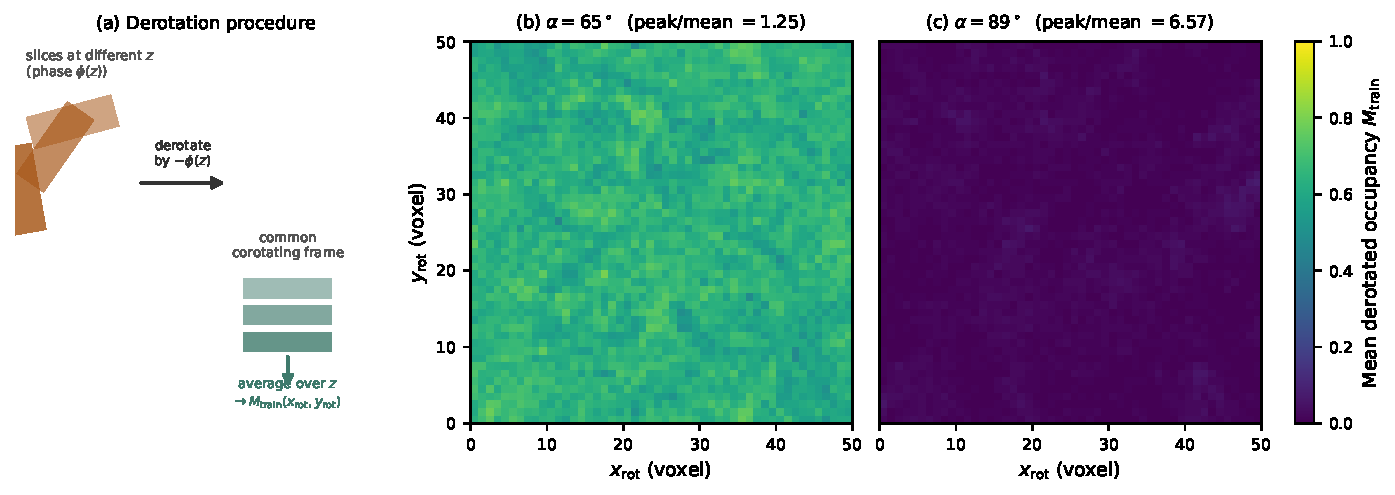
\includegraphics[width=0.85\linewidth]{corotating_oracle_maps}
  \caption{%
    The corotating-frame template itself is visually uninformative in
    both limits, which is why no fixed-template predictor can beat the
    bulk filling fraction (Table~\ref{tab:oracle}).
    (a) Schematic of the derotation procedure (conceptual diagram): each
    $z$-slice is derotated by the local helix phase $-\phi(z)$ into a
    common corotating frame, then averaged over $z$ to give
    $M_{\mathrm{train}}(x_{\mathrm{rot}},y_{\mathrm{rot}})$.
    (b),(c) The resulting mean derotated occupancy map for the two
    extreme peak-to-mean angles, $\dang = 65^{\circ}$ (peak/mean $=1.25$)
    and $\dang = 89^{\circ}$ (peak/mean $=6.57$), accumulated over
    training slices $z \in [0,121]$.
    Neither map shows a coherent, learnable spatial template: the
    $65^{\circ}$ map is uncorrelated speckle around a high bulk
    occupancy, and the $89^{\circ}$ map's higher peak-to-mean ratio
    reflects a lower overall occupancy rather than emergent structure.
  }
  \label{fig:corotating_maps}
\end{figure}
Empirically, then, the time-averaged derotated occupancy map carries no
fixed spatial template that improves on the bulk filling fraction for
\emph{this} simulator's pooled stochastic-nucleation protocol: the
individual column positions are set independently in each run, so a
coordinate-conditioned predictor of the form $f(x,y,z,\dang)\to I$ has no
realization-invariant target to recover beyond the uniform-occupancy
baseline.
We emphasise that this is an empirical finding for the present simulator
and the present corotating protocol, \emph{not} a general proof that no
model can ever fit a voxel field: a single realised field is deterministic
once generated and could in principle be memorised, but such an absolute
fixed-template fit would not transfer to an independently nucleated run.
The result bounds only \emph{absolute, fixed spatial templates}; it does
not rule out probabilistic or generative models, latent-seed-conditioned
fields, distributional prediction, or equivariant architectures that target
the statistics rather than the absolute positions.  The defensible
conclusion is that absolute fixed spatial templates do not transfer between
the tested independently nucleated realizations, whereas selected ensemble
statistics (Section~\ref{ssec:nif_corr}) are far more reproducible.
In experimental terms, this is equivalent to finding that, after derotation
into the corotating frame, the column positions in one GLAD film provide no
template that predicts the column positions of a nominally identical film
grown in a separate run.

\begin{table}[htbp]
  \centering
  \caption{%
    Corotating-frame oracle.
    $M_{\mathrm{train}}$: mean derotated occupancy from training
    slices $z \in [0, 121]$.
    $\Delta_{\mathrm{in}}$/$\Delta_{\mathrm{ho}}$: IoU gain above the
    all-positive baseline ($\mathrm{IoU}=f$) on training / holdout
    ($z \in [121, 151]$) regions.
    All gains are $\leq 0$, showing that the best fixed mean-template
    baseline (the mean derotated map, thresholded) does not exceed the
    all-positive baseline for this simulator's pooled stochastic-nucleation
    protocol. $f_{\mathrm{train}}$/$f_{\mathrm{hold}}$ here use the
    $z\in[0,121]$/$[121,151]$ voxel-index convention of this table only;
    the companion study \citep{companionP2} reports occupied fractions
    over a different, full-height $z$-range at the same $\dang$, so its
    numeric values (e.g.\ $0.177$ vs.\ this table's $0.126$ at
    $\dang=85^{\circ}$) are not directly comparable without accounting for
    that convention difference.
    An IoU gain of zero means that the best fixed spatial template does no
    better than the trivial all-positive segmentation---equivalent to
    finding that individual column positions carry no recoverable fixed
    spatial pattern in the derotated image of this film.  This bounds fixed
    templates only, not probabilistic or equivariant predictors of the
    column statistics.
  }
  \label{tab:oracle}
  \begin{tabular}{cccccc}
    \toprule
    $\dang$ ($^{\circ}$) & $f_{\mathrm{train}}$ & $f_{\mathrm{hold}}$ &
    $\Delta_{\mathrm{in}}$ & $\Delta_{\mathrm{ho}}$ & peak/mean \\
    \midrule
    65 & 0.635 & 0.585 & $\phantom{-}0.000$  & $\phantom{-}0.000$   & 1.25 \\
    70 & 0.502 & 0.467 & $\phantom{-}0.000$  & $\phantom{-}0.000$   & 1.37 \\
    75 & 0.292 & 0.282 & $\phantom{-}0.000$  & $\phantom{-}0.000$   & 1.58 \\
    80 & 0.233 & 0.230 & $\phantom{-}0.000$  & $\phantom{-}0.000$   & 1.65 \\
    85 & 0.126 & 0.130 & $\phantom{-}0.000$  & $\phantom{-}0.000$   & 2.49 \\
    87 & 0.076 & 0.075 & $-0.0001$           & $-0.0006$            & 2.63 \\
    89 & 0.012 & 0.007 & $-0.0008$           & $-0.0024$            & 6.57 \\
    \bottomrule
  \end{tabular}
\end{table}

\subsection{Two-point pair correlation and CorrNIF interpolation}
\label{ssec:nif_corr}

Since individual voxel occupancies are stochastic, we shift the target
to the \textit{ensemble-level} statistical morphology: the normalised
two-point pair correlation $h_g(r;\dang)$.
This real-space descriptor is related, through Fourier transformation, to
the structure-factor $S(\mathbf{q})$ accessible by small-angle or
grazing-incidence X-ray scattering (SAXS/GISAXS) on nanostructured films
\citep{renaud2009gisaxs};
the connection is subject to the form factor of the columns, their
orientation distribution, and instrumental resolution, so $h_g(r)$ is not
itself a directly measured pair-distribution function but a quantity
Fourier-conjugate to the measurable scattering intensity, in the same
sense as the pair-distribution function of a simple liquid is
Fourier-conjugate to its static structure factor \citep{hansen2013theory}.
It quantifies how the correlation of column material decays with radial
distance~$r$ from a reference point in the transverse plane.
Unlike individual column positions (Section~\ref{ssec:nif_voxel}),
$h_g(r;\dang)$ is reproducible at the descriptor level across
independent simulation runs at a given $\dang$, and varies smoothly with deposition angle.
We verify this reproducibility directly using the three independent
seeds available at $\dang = 80^{\circ}$ and $85^{\circ}$, computing
$h_g(r)$ separately for each seed.  To avoid the optimistic bias of
comparing each seed only against a mean that contains it, we report
\emph{independent} estimators: the mean pairwise (seed-to-seed)
root-mean-square deviation is $0.0077$ at $80^{\circ}$ and $0.0090$ at
$85^{\circ}$, and the leave-one-seed-out deviation (each seed versus the
mean of the other two) is $0.0066$ and $0.0078$, respectively (maximum
pointwise standard deviation $0.010$ at $80^{\circ}$, $0.007$ at
$85^{\circ}$).  The self-inclusive deviation used in earlier drafts
($0.002$--$0.007$) understates the true variability.
The \textsc{CorrNIF} leave-one-angle-out error at these angles
(RMSE $\approx 0.011$, Table~\ref{tab:looa}) is therefore comparable to,
and about $1.2$--$1.7\times$ above, the independent seed-to-seed scatter:
the curve is a genuinely reproducible ensemble descriptor, and the emulator
reproduces it to within a small multiple of the simulator's own run-to-run
variability.
The single-seed configurations at the remaining angles are used as-is;
extending the three-seed test to the full angular range is identified as
future work.

\textit{Definition.}
After bilinear derotation the corotating-frame field is a \emph{continuous}
occupancy field $J(\mathbf{r}) \in [0,1]$ with mean
$f = \langle J \rangle$ (equal to the binary filling fraction up to the
interpolation error).  We use the normalised covariance
\begin{equation}
  C(r) = \langle J(\mathbf{x})\,J(\mathbf{x}+r)\rangle,
  \label{eq:pair_corr}
\end{equation}
\begin{equation}
  h_g(r) = \frac{C(r) - f^2}{C(0) - f^2},
  \qquad h_g(0) = 1,
  \label{eq:hg_norm}
\end{equation}
where $C(0)=\langle J^2\rangle$ is read empirically from the zero-lag
pixel.  This continuous-covariance form (a standard normalised covariance)
guarantees $h_g(0)=1$ \emph{without} requiring the binary identity
$\langle J^2\rangle=\langle J\rangle$, which the interpolated field does not
satisfy: empirically $C(0)/f^2$ ranges from $1.35$ ($65^{\circ}$) to $59$
($89^{\circ}$) and differs by $15$--$25\%$ from the binary value $1/f$ at
every angle, confirming that the normalisation must use the measured
variance rather than $1/f$.
Contrary to a naive expectation, $h_g(r)$ is \emph{not} confined to
$[0,1]$: $C(r)$ may fall below $f^2$ where the arrangement is anticorrelated,
so $h_g(r)$ takes small negative values at finite separation (down to
$\approx-0.013$ at $80$--$89^{\circ}$ here).
For an infinite statistically homogeneous system the correlation is
expected to approach zero at large separation; the present periodic domain
only samples $r\le L/2$, so the long-range value is not a measured
$h_g(\infty)=0$ but a finite-box estimate.
Equivalently, $h_g(r)=[C(r)-f^2]/[C(0)-f^2]$ is the connected correlation
normalised by its own zero-lag value; its radial \emph{shape} remains
numerically sensitive as $f\to 0$ ($\dang\to 90^{\circ}$), where both
$C(r)-f^2$ and $C(0)-f^2$ become small.  By construction $h_g(0)=1$ for all
$f$, so $h_g(0)$ encodes no filling-fraction information; the filling
fraction is supplied separately from the binary field.

$h_g(r;\dang)$ is computed in the corotating frame using bilinear
derotation and the FFT-based circular autocorrelation, then
radially averaged over the transverse plane
(full pipeline in Section~\ref{ssec:nif_methods}).
Figure~\ref{fig:nif_corr} shows the resulting curves for all
seven configurations.
\emph{Derotation convention.}  The curves shown, the cross-seed statistics,
the leave-one-angle-out \textsc{CorrNIF} retraining, and the corrected
$72^{\circ}$ baselines (Section~\ref{ssec:nif_prospective}) all use the
periodic-wrap derotation and the continuous-covariance normalisation of
Eqs.~\ref{eq:pair_corr}--\ref{eq:hg_norm}.  Negative values of $h_g$ are
retained rather than clipped.

\begin{figure}[htbp]
  \centering
  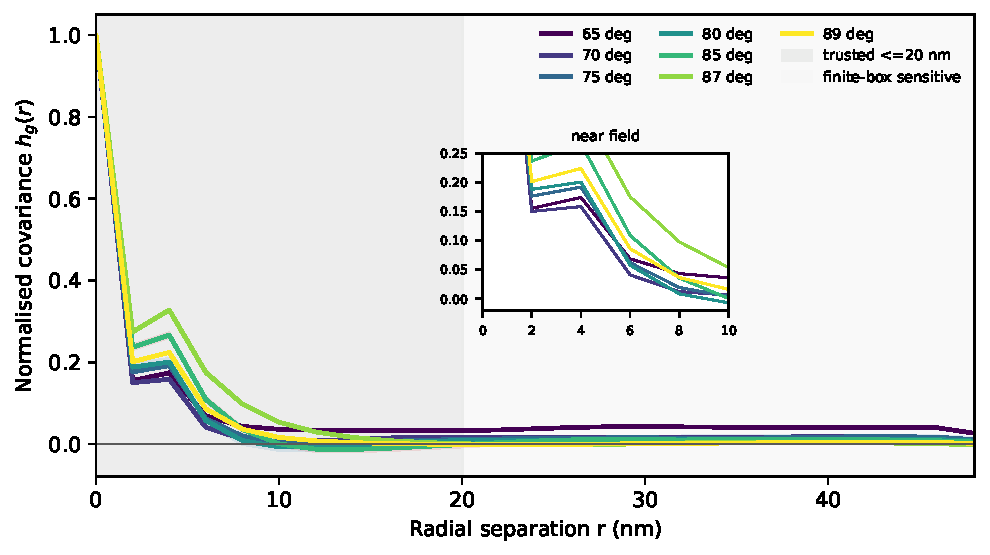
\includegraphics[width=0.85\linewidth]{nif_pair_correlation}
  \caption{%
    The column-arrangement statistics change smoothly and systematically
    with deposition angle, unlike the individual column positions
    themselves, making this curve a promising reproducible target for
    interpolation across angles.
    Normalised two-point pair correlation $h_g(r;\dang)$ in the
    corotating frame, for all seven deposition angles
    ($\dang = 65^{\circ}$--$89^{\circ}$, viridis colour scale; dense to sparse).
    This real-space descriptor is Fourier-conjugate to the structure factor
    $S(\mathbf{q})$ probed by SAXS/GISAXS: it quantifies how the correlation
    of column material decays with radial distance $r$, normalised to unity
    at $r = 0$.
    Curves differ systematically in amplitude and tail decay across $\dang$,
    providing the smooth signal for pair-correlation emulation; shaded
    uncertainty bands are shown where replicated corrected curves are
    available.
    All curves satisfy $h_g(0)=1$ by construction and take small negative
    values at finite $r$ where the arrangement is anticorrelated; the
    long-range tail is a finite-box ($r\le L/2$) estimate, not a measured
    $h_g(\infty)=0$.
  }
  \label{fig:nif_corr}
\end{figure}

\textit{\textsc{CorrNIF} architecture} (see Section~\ref{ssec:nif_methods}
for full specification).
A compact NIF maps $(\dang_{\rm norm}, r_{\rm norm}) \to h_g$,
with a random Fourier encoder on $r$ ($n_{\rm freq}=12$, $\sigma_r=2$
\citep{tancik2020}), three hidden layers (width~64, SiLU),
and angle conditioning (FiLM) on $\dang$.

\textit{LOOA validation.}
In a seven-fold leave-one-angle-out (LOOA) experiment, \textsc{CorrNIF} is
trained on six angles and used to predict $h_g(r;\dang_{\mathrm{held}})$.
Figure~\ref{fig:nif_looa} shows LOOA predictions against the reference curves.
Results are summarised in Table~\ref{tab:looa}.

\begin{figure}[htbp]
  \centering
  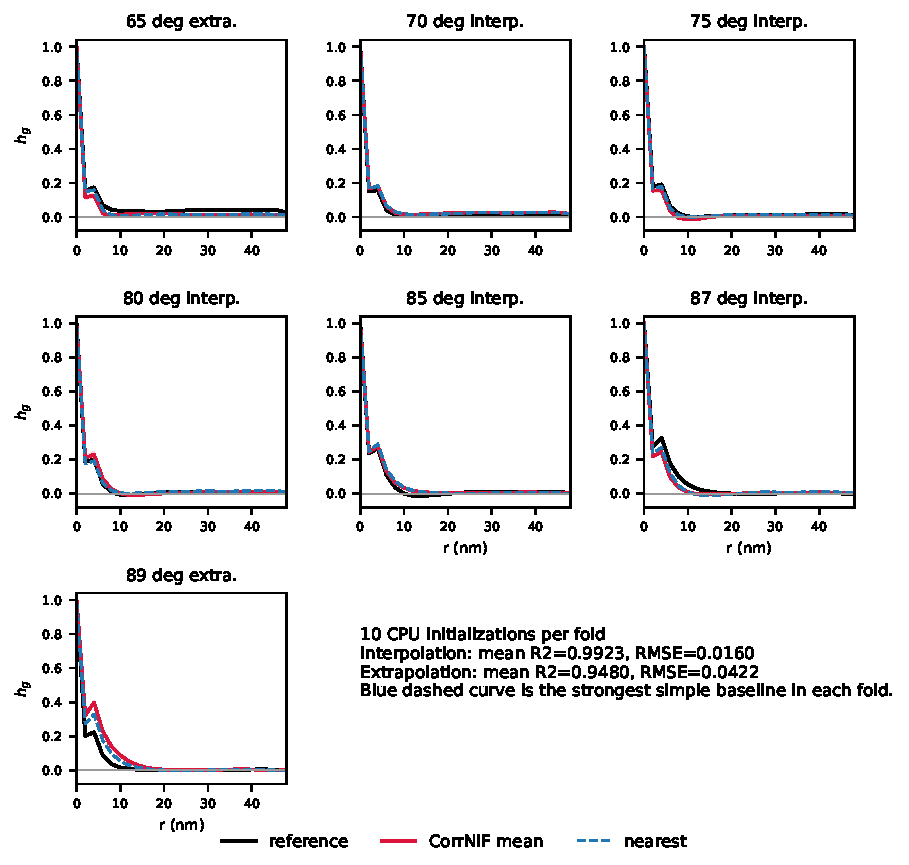
\includegraphics[width=\linewidth]{nif_looa_predictions}
  \caption{%
    The trained emulator successfully reconstructs the column-arrangement
    statistics at deposition angles it never saw during training, but so
    do much simpler interpolation methods, so its practical value lies in
    convenience rather than superior accuracy.
    Leave-one-angle-out \textsc{CorrNIF} predictions of
    $h_g(r;\dang_{\mathrm{held}})$.
    In each panel, the emulator was trained on the six remaining
    deposition angles and had no access to the held-out angle---analogous
    to fitting an optical dispersion model to six incidence-angle spectra
    and predicting the seventh.
    Black solid lines: corrected reference curves computed from voxel data.
    Crimson solid lines and bands: mean and one-standard-deviation range of
    ten independently initialised \textsc{CorrNIF} trainings.
    Blue dashed lines: the strongest simple baseline for the corresponding
    fold, evaluated against the same corrected target.
    Panel labels identify interpolation and extrapolation folds.  The emulator
    interpolates the interior folds accurately but does not outperform the
    strongest simple baselines on accuracy.
  }
  \label{fig:nif_looa}
\end{figure}

\begin{table}[htbp]
  \centering
  \caption{%
    Leave-one-alpha-out (LOOA) performance of \textsc{CorrNIF} versus
    interpolation baselines evaluated on the \emph{same corrected} folds:
    nearest-neighbour (NN, copy the training curve at the closest $\dang$),
    linear blend (interpolate/extrapolate between the two nearest training
    angles), Gaussian-process regression (GP, squared-exponential kernel,
    fitted per radial bin), and monotone cubic (PCHIP) interpolation along
    $\dang$.
    $R^2$: coefficient of determination on the held-out curve
    $h_g(r;\dang_{\mathrm{held}})$.
    The two sweep-boundary folds ($65^{\circ}$, $89^{\circ}$) are
    \emph{extrapolation}; the five interior folds are \emph{interpolation}
    and are aggregated separately.
    \textsc{CorrNIF} entries are the mean predictions from ten independent
    neural initialisations.  \textsc{CorrNIF} does not exceed the best simple
    baselines on accuracy: its interior mean $R^2$ ($0.9923$) is numerically
    comparable to linear and PCHIP ($0.9928$), while the extrapolation mean
    drops to $0.9480$.  The half-width error
    $|\Delta d_{\mathrm{col}}| = 2|\Delta r_{1/2}|$ is omitted because
    $r_{1/2}\approx\SI{1.2}{nm}\lesssim 1$~vox at all angles, below the
    \SI{2}{nm} voxel resolution, so it is a sub-voxel curve-shape diagnostic
    rather than a physical column diameter.
  }
  \label{tab:looa}
  \begin{tabular}{lccccc}
    \toprule
    $\dang_{\mathrm{held}}$ ($^{\circ}$)
      & \textsc{CorrNIF}
      & NN
      & Linear
      & GP
      & PCHIP \\
    \midrule
    \multicolumn{6}{l}{\emph{Interior folds (interpolation)}}\\
    70 & 0.9969 & 0.9872 & 0.9960 & 0.5602 & 0.9969 \\
    75 & 0.9954 & 0.9973 & 0.9994 & 0.8604 & 0.9987 \\
    80 & 0.9970 & 0.9989 & 0.9974 & 0.9283 & 0.9983 \\
    85 & 0.9953 & 0.9801 & 0.9932 & 0.9830 & 0.9899 \\
    87 & 0.9768 & 0.9810 & 0.9777 & 0.9852 & 0.9802 \\
    \textit{Interior mean} & \textit{0.9923} & \textit{0.9889} & \textit{0.9928} & \textit{0.8634} & \textit{0.9928} \\
    \textit{Interior median} & \textit{0.9954} & \textit{0.9872} & \textit{0.9960} & \textit{0.9283} & \textit{0.9969} \\
    \midrule
    \multicolumn{6}{l}{\emph{Boundary folds (extrapolation)}}\\
    65 & 0.9805 & 0.9865 & 0.9865 & -3.5859 & 0.9754 \\
    89 & 0.9155 & 0.9699 & 0.9699 & 0.8431 & 0.9267 \\
    \textit{Boundary mean} & \textit{0.9480} & \textit{0.9782} & \textit{0.9782} & \textit{-1.3714} & \textit{0.9511} \\
    \midrule
    \textbf{All-fold mean} & \textbf{0.9796} & \textbf{0.9858} & \textbf{0.9886} & \textbf{0.2249} & \textbf{0.9809} \\
    \bottomrule
  \end{tabular}
  \par\smallskip
  \noindent\small All $R^2$ values are coefficients of determination on the
  held-out curve. Interior interpolation is accurate and method-insensitive
  ($R^2 \approx 0.99$ for CorrNIF, linear, and PCHIP); boundary extrapolation
  degrades, especially for \textsc{CorrNIF} at $89^{\circ}$ ($R^2 = 0.916$).
  The per-bin GP baseline is unstable for the corrected target under this
  small-angle training set, especially at the $65^{\circ}$ boundary. Cubic
  spline interpolation (not shown) gives all-fold mean $R^2 = 0.957$.
\end{table}

The corrected LOOA results confirm that $h_g(r;\dang)$ is a smoothly
learnable function of $\dang$ in the interior of the angle sweep.
For the five interpolation folds, \textsc{CorrNIF} reaches mean
$R^2 = 0.9923$ (median $0.9954$, worst case $0.9768$).
Crucially, this smoothness is not unique to the neural emulator: on the
same corrected folds, nearest-neighbour, linear, and PCHIP baselines also
reproduce the held-out curves about equally well (Table~\ref{tab:looa}).
We therefore do not claim that \textsc{CorrNIF} interpolates
\emph{more accurately} than these simpler methods---it does not.
Its advantage is qualitative: it provides a single differentiable,
continuous, multi-output representation $h_g(r;\dang)$ that can be queried
and differentiated at arbitrary $(\dang,r)$ and extended to additional
outputs, which is convenient for downstream gradient-based optimisation but
not necessary for the present interpolation task, where a simpler method
would suffice.
The extrapolation folds are weaker: the \textsc{CorrNIF} boundary mean is
$R^2 = 0.9480$, with the lowest performance at $\dang = 89^{\circ}$
($R^2 = 0.9155$), the most extreme sparse-boundary case in the sweep.
This underscores that no single interpolator dominates and that the choice
should be driven by the downstream use rather than by held-out accuracy
alone.

\subsection{Prospective interpolation at \texorpdfstring{$\dang=72^{\circ}$}{alpha=72 deg}}
\label{ssec:nif_prospective}

As a prospective check, we query \textsc{CorrNIF}---trained on all seven
existing configurations $\dang \in \{65,70,75,80,85,87,89\}^{\circ}$---at the
deposition angle $\dang = 72^{\circ}$, which is genuinely absent from the
training set.
This point lies $40\%$ of the way between the nearest training neighbours
$70^{\circ}$ and $75^{\circ}$, making it a mid-range interpolation rather than
an extrapolation. Figure~\ref{fig:calib_grid} shows this calibration
design directly.

\begin{figure}[htbp]
  \centering
  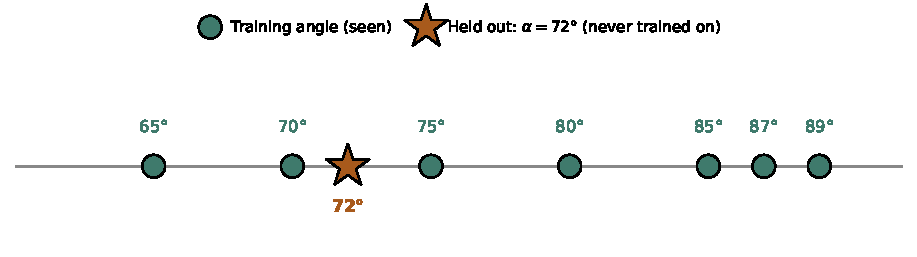
\includegraphics[width=0.78\linewidth]{calibration_grid_72}
  \caption{%
    The $72^{\circ}$ test is a genuine blind interpolation, not a
    relabelled training point: this angle contributes nothing to
    \textsc{CorrNIF}'s parameters before the comparison in
    Figure~\ref{fig:nif_prospective} is made.
    \textsc{CorrNIF}'s training grid (green circles) versus the held-out
    prospective test angle (orange star, $\dang=72^{\circ}$), which is
    excluded from training and from all main-dataset descriptive
    analyses (Section~\ref{ssec:params}).
  }
  \label{fig:calib_grid}
\end{figure}

Figure~\ref{fig:nif_prospective} compares the corrected \textsc{CorrNIF}
prediction at $72^{\circ}$ against the dedicated reference simulation and
the strongest simple baseline, a linear blend
$h_{\rm lin}(r;72^{\circ}) = 0.6\,h_g(r;70^{\circ}) + 0.4\,h_g(r;75^{\circ})$.
The \textsc{CorrNIF} prediction interpolates smoothly between the two
neighbouring training curves but is not more accurate than this linear
baseline on the corrected target.

\begin{figure}[htbp]
  \centering
  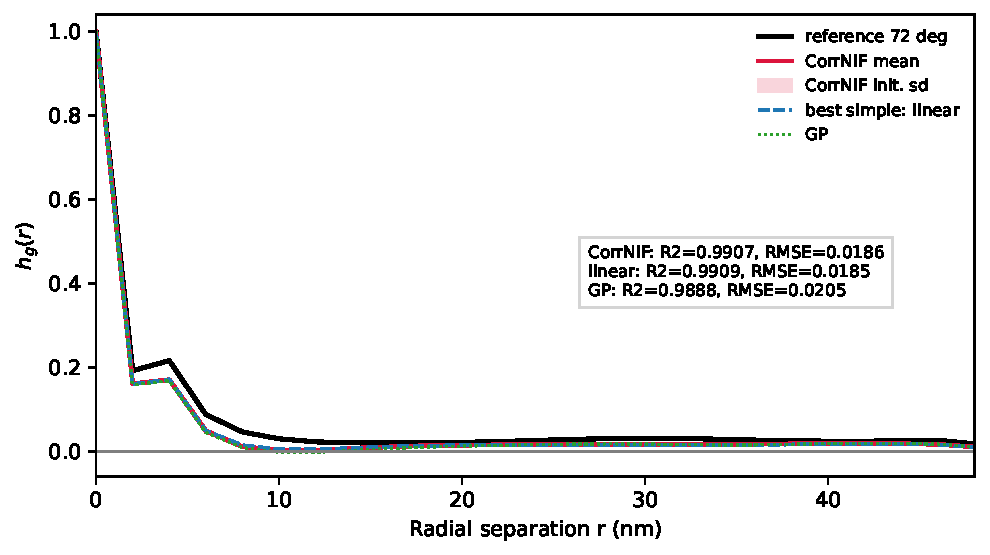
\includegraphics[width=0.85\linewidth]{nif_alpha72_prospective}
  \caption{%
    A genuinely new deposition angle, never used for training and
    subsequently confirmed by an independent simulation, is predicted
    accurately by the emulator---though again no more accurately than a
    simple linear interpolation between the two nearest trained angles.
    \textsc{CorrNIF} prospective prediction versus dedicated reference simulation
    at $\dang = 72^{\circ}$ (absent from the training set).
    Black solid: reference simulation $h_g(r;\,72^{\circ})$
    ($h = 300$~nm, $68\times10^6$ atoms).
    Crimson solid and shaded band: mean and one-standard-deviation range of
    ten \textsc{CorrNIF} initialisations ($R^2 = 0.9907$ for the mean curve).
    Orange dotted: linear-blend baseline ($R^2 = 0.9909$).
    Green dash-dotted: GP baseline ($R^2 = 0.9888$).
    The comparison uses the same corrected periodic-wrap,
    continuous-covariance target for every method.
  }
  \label{fig:nif_prospective}
\end{figure}

To validate this prospective prediction, a dedicated simulation at
$72^{\circ}$ was subsequently run under identical conditions ($300$~nm,
$68\times10^6$ deposited atoms).
Evaluated against this dedicated reference simulation on the corrected
continuous-covariance target, \textsc{CorrNIF} gives $R^2 = 0.9907$
(RMSE $0.0186$), while the linear blend gives $R^2 = 0.9909$
(RMSE $0.0185$), the best of the simple methods tested here.  Nearest
neighbour, PCHIP, cubic spline, and GP give $R^2=0.9882$, $0.9902$,
$0.9904$, and $0.9888$, respectively.  We therefore do \emph{not} claim
that \textsc{CorrNIF} captures a non-linear $\dang$-dependence of the
correlation tail that the simple interpolators cannot reproduce: for this
single point they are numerically comparable.
The result confirms that \textsc{CorrNIF} generalises to a genuinely unseen
interpolation point, with no demonstrated accuracy advantage over simple
interpolation.

\subsection{Demonstrating the differentiability advantage: gradient-based recovery of \texorpdfstring{$\dang$}{alpha}}
\label{ssec:nif_gradient_demo}

Sections~\ref{ssec:nif_corr}--\ref{ssec:nif_prospective} establish that
\textsc{CorrNIF}'s only demonstrated advantage over simple, non-differentiable
baselines is qualitative: because it is a continuous, differentiable function
of $\dang$, it supports gradient-based queries that nearest-neighbour,
linear, and PCHIP interpolation do not. We demonstrate this advantage
directly with a minimal inverse-design experiment, rather than leaving it as
an unexercised claim.

\textit{Task.} Treat the dedicated-simulation-confirmed pair-correlation
curve at $\dang=72^{\circ}$ (Section~\ref{ssec:nif_prospective}, genuinely
absent from \textsc{CorrNIF}'s training set) as an observed target, and
recover the deposition angle that produced it by gradient descent through
the frozen, already-trained \textsc{CorrNIF} model---treating $\dang$ itself
as the only free parameter, with model weights held fixed. This mirrors a
practical use case: given a desired or measured correlation shape, find the
process angle that reproduces it without re-running the ballistic simulator
or performing a discrete grid search.

\textit{Procedure and cross-check.} Starting from five deliberately
mismatched initial guesses spanning the training range
($\dang_0 \in \{65,70,80,85,89\}^{\circ}$), we minimise the mean-squared
error between \textsc{CorrNIF}'s output and the target curve using Adam
(300 steps, learning rate $0.05$ on the normalised angle). As an independent
correctness check, we also compute the loss on an exhaustive fine grid
($0.005^{\circ}$ resolution) over the full training range.

\begin{figure}[htbp]
  \centering
  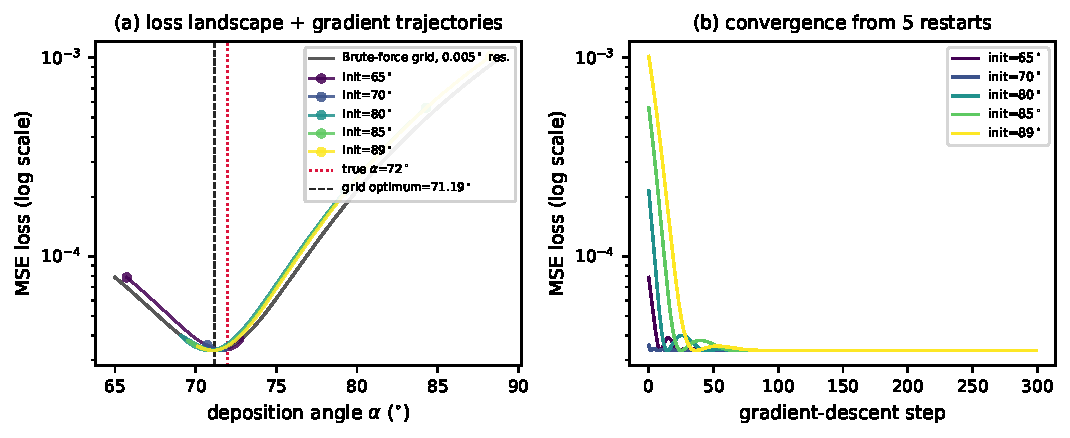
\includegraphics[width=\linewidth]{corrnif_gradient_inverse_demo}
  \caption{%
    Gradient descent through the frozen \textsc{CorrNIF} model recovers the
    same angle from every tested starting point, and that angle matches an
    independent exhaustive grid search to within $0.002^{\circ}$---direct
    evidence that the differentiability claimed for \textsc{CorrNIF} is
    usable, not just structurally present.
    (a)~Brute-force loss landscape $L(\dang)$ (grey) with the five
    gradient-descent trajectories overlaid, all converging to the same
    minimum regardless of starting point.
    (b)~Per-restart loss-versus-iteration convergence, all five restarts
    reaching the same final loss within 300 steps.
  }
  \label{fig:corrnif_gradient_demo}
\end{figure}

\textit{Result.} All five restarts converge to the identical recovered angle,
$\dang_{\rm rec} = 71.183^{\circ}$ (standard deviation across restarts
$<10^{-4}\,^{\circ}$), regardless of starting point---including restarts
initialised on the opposite side of the true angle from each other
(Figure~\ref{fig:corrnif_gradient_demo}). This matches the independent
brute-force grid optimum, $71.185^{\circ}$, to within $0.002^{\circ}$,
confirming that gradient descent converges to the same optimum as exhaustive
search rather than to an unrelated stationary point. Each restart converges
in under 4 seconds on CPU (300 Adam steps); the one-time cost of training
\textsc{CorrNIF} itself is under one minute. We report this timing only to
show the inverse query itself is cheap once trained, not as a claim that
training plus inverse recovery is faster than a single ballistic simulation
at a known angle.

We do \emph{not} claim this recovers the true angle exactly: the recovered
$71.183^{\circ}$ differs from the actual deposition angle,
$\dang=72^{\circ}$, by $0.82^{\circ}$. We do not claim this residual is
formally comparable in magnitude to the curve-fit error reported for this
same target curve in Section~\ref{ssec:nif_prospective}
($R^2=0.9907$, RMSE~$=0.0186$): an angular residual (degrees) and a
curve-shape RMSE (dimensionless $h_g$ units) are different quantities, and
no error-propagation relating them is derived here. Qualitatively, the
$0.82^{\circ}$ residual is small relative to the $5^{\circ}$ spacing
between the nearest training angles ($70^{\circ}$, $75^{\circ}$), consistent
with the inverse recovery being limited by the same finite-capacity,
finite-training-grid interpolation imperfection as the forward prediction,
rather than by a failure of the optimisation procedure itself, which is
independently validated by the exact grid-search agreement above. The
demonstration therefore substantiates the differentiability advantage as
claimed: a genuine gradient-based query is usable in practice, at a
precision commensurate with, and no worse than, \textsc{CorrNIF}'s already
established forward-interpolation accuracy.

\subsection{Effective optical properties: a loss-aware Maxwell-Garnett screening illustration}
\label{ssec:nif_optical}

This subsection addresses \textbf{Q4}.
We compute effective optical constants from the filling fractions
$f(\dang)$ using the aligned-cylinder Maxwell-Garnett (MG) effective-medium
approximation \citep{maxwell1904} (see Section~\ref{ssec:nif_methods}
for the model setup and its limitations).
As a sensor-design hypothesis-generation illustration only, we take tungsten columns
($\varepsilon_{\mathrm{W}} = 4.41 + 19.60i$ at $\lambda \approx \SI{500}{nm}$,
i.e.\ $n=3.5$, $k=2.8$ \citep{palik1985}) in vacuum, with structural
$f(\dang)$ extracted from the Cu GLAD simulations.  This screening calculation uses the same $R=\SI{0.128}{nm}$ Cordero
covalent-radius \citep{cordero2008} campaign as the void-fraction results
of Section~\ref{sec:results_openness} (Table~\ref{tab:params}), whereas
the PCA and pair-correlation descriptor-space results
(Sections~\ref{ssec:pca}, \ref{ssec:nif_methods}) draw on the
separately-described extended, repeated-seed dataset at $R=\SI{0.1}{nm}$;
the two radii give systematically slightly different filling fractions
(void fraction $\sim 0.3$--$0.5$ percentage points lower at
$R=\SI{0.128}{nm}$), which does not change any qualitative conclusion
drawn here but should not be conflated with the single-realization
void-fraction numbers reported in Section~\ref{sec:results_openness}.
Two further caveats govern the interpretation of this calculation.
First, the filling fraction is definition-dependent: the bead-sphere solid
fraction $1-\bsP$ and the thresholded voxel occupancy $f_{\rho>0.5}$ differ
by up to a factor of four at low $\dang$ (e.g.\ $0.115$ vs $0.492$ at
$65^{\circ}$; Table~\ref{tab:fcompare}), and the thresholded occupancy is
itself sensitive to the Gaussian voxelisation kernel and the $0.5$ threshold
rather than being a physical material volume fraction.  Second, the columns
are strongly absorbing, so the extraordinary polarisation carries a large
extinction $k_e$ that must be reported alongside $\Delta n$.
We therefore present the optical results as an illustrative, definition- and
material-dependent screening calculation, not a quantitative design
prediction, and report both filling-fraction conventions.

The ordinary index $n_o$ (transverse polarisation,
cylindrical inclusion geometry) is obtained from:
\begin{equation}
  \varepsilon_o = \varepsilon_h\,
  \frac{(\varepsilon_c + \varepsilon_h) + f(\varepsilon_c - \varepsilon_h)}
       {(\varepsilon_c + \varepsilon_h) - f(\varepsilon_c - \varepsilon_h)},
  \label{eq:mg_transverse}
\end{equation}
and the extraordinary index $n_e$ (longitudinal, Wiener parallel limit) from:
\begin{equation}
  \varepsilon_e = f\,\varepsilon_c + (1-f)\,\varepsilon_h,
  \label{eq:mg_parallel}
\end{equation}
where $\varepsilon_c$ is the column dielectric function and
$\varepsilon_h = 1$ (vacuum host).
The form birefringence is $\Delta n = |n_e - n_o|$.

Figure~\ref{fig:nif_optical} and Table~\ref{tab:mg} give the results.

\begin{figure}[htbp]
  \centering
  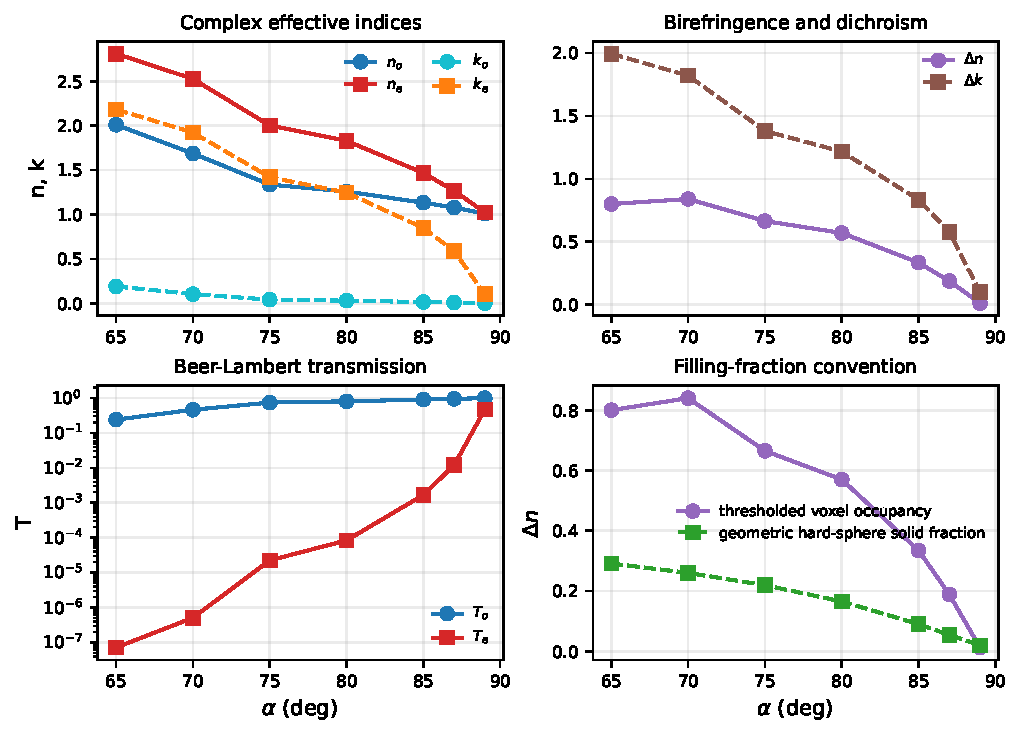
\includegraphics[width=\linewidth]{nif_optical_properties}
  \caption{%
    A large apparent form birefringence at moderate obliquity is
    accompanied by near-total absorption of the extraordinary
    polarisation, and the apparent optimum angle is itself an artefact of
    how the solid filling fraction is defined---so this screening
    illustrates the morphology-to-optics pathway without identifying a
    usable polarimetric design window.
    Loss-aware aligned-cylinder Maxwell-Garnett optical screening of a
    W-column film versus $\dang$ (illustrative material substitution; see
    Section~\ref{ssec:nif_methods}).
    (a)~Full complex effective indices for the thresholded-occupancy
    filling fraction: ordinary $n_o$ and extraordinary $n_e$ (solid),
    ordinary $k_o$ and extraordinary $k_e$ (dashed).  The extraordinary
    extinction $k_e$ is of order unity.
    (b)~Form birefringence $\Delta n=|n_e-n_o|$ and dichroism
    $\Delta k=|k_e-k_o|$; the dichroism exceeds the birefringence across the
    sweep.
    (c)~Beer--Lambert intensity transmission of the two eigenpolarisations
    through the \SI{300}{nm} film (log scale): the extraordinary
    transmission $T_e$ stays far below $1\%$ throughout the high-$\Delta n$
    range, i.e.\ the extraordinary eigenstate is essentially fully absorbed.
    (d)~$\Delta n$ computed with the two filling-fraction conventions: the
    apparent maximum near $65^{\circ}$ (thresholded occupancy
    $f_{\rho>0.5}$, $\Delta n = 0.839$) disappears for the geometric hard-sphere solid fraction
    $1-\bsP$, which decays monotonically.
    No polarimetric design window is claimed; the authoritative tabulated
    values are in Tables~\ref{tab:fcompare} and~\ref{tab:mg}.
  }
  \label{fig:nif_optical}
\end{figure}

\begin{table}[htbp]
  \centering
  \caption{%
    Filling-fraction reconciliation.  $\bsP$: bead-sphere void fraction
    (Eq.~\ref{eq:bead_sphere}); $1-\bsP$: bead-sphere solid fraction;
    $f_{\rho>0.5}$: thresholded voxel occupancy used in the optical
    calculation.  The two solid-fraction measures differ by up to a factor
    of four and are not interchangeable; $f_{\rho>0.5}$ depends on the
    voxelisation kernel and threshold and is not a physical material volume
    fraction.
  }
  \label{tab:fcompare}
  \begin{tabular}{ccccc}
    \toprule
    $\dang$ ($^{\circ}$) & $\bsP$ (\%) & $1-\bsP$ & $f_{\rho>0.5}$ &
    $f_{\rho>0.5}/(1-\bsP)$ \\
    \midrule
    65 & 88.5 & 0.115 & 0.492 & 4.3 \\
    70 & 89.5 & 0.105 & 0.409 & 3.9 \\
    75 & 90.9 & 0.091 & 0.348 & 3.8 \\
    80 & 92.7 & 0.073 & 0.197 & 2.7 \\
    85 & 95.3 & 0.047 & 0.113 & 2.4 \\
    87 & 96.6 & 0.034 & 0.070 & 2.0 \\
    89 & 98.1 & 0.019 & 0.011 & 0.6 \\
    \bottomrule
  \end{tabular}
\end{table}

\begin{table}[htbp]
  \centering
  \caption{%
    Aligned-cylinder Maxwell-Garnett effective optical constants
    \citep{maxwell1904} for a high-index columnar film
    ($\varepsilon_{\mathrm{W}} = 4.41 + 19.60i$, $\lambda \approx \SI{500}{nm}$
    \citep{palik1985}, vacuum host), using the thresholded voxel occupancy
    $f = f_{\rho>0.5}$.  Both polarisations are now reported as full complex
    indices.  $n_o,k_o$: ordinary index and extinction; $n_e,k_e$:
    extraordinary index and extinction; $\Delta n=|n_e-n_o|$;
    $T_e$: extraordinary intensity transmission through the \SI{300}{nm}
    film (Beer--Lambert screening, normal incidence, interfaces neglected).
    The large $k_e$ and near-zero $T_e$ across the high-$\Delta n$ range show
    that the extraordinary eigenstate is essentially fully absorbed; the
    figures are an illustrative screening calculation only
    (see Table~\ref{tab:fcompare} for the filling-fraction caveat).
  }
  \label{tab:mg}
  \footnotesize
  \begin{tabular}{ccccccccc}
    \toprule
    $\dang$ ($^{\circ}$) & $f$ & $n_o$ & $k_o$ & $n_e$ & $k_e$ & $\Delta n$ & $\Delta k$ & $T_e$ \\
    \midrule
    65 & 0.492 & 1.679 & 0.102 & 2.518 & 1.914 & 0.839 & 1.81 & $5\times10^{-7}$ \\
    70 & 0.409 & 1.522 & 0.070 & 2.320 & 1.728 & 0.798 & 1.66 & $2\times10^{-6}$ \\
    75 & 0.348 & 1.421 & 0.053 & 2.161 & 1.576 & 0.740 & 1.52 & $7\times10^{-6}$ \\
    80 & 0.197 & 1.214 & 0.024 & 1.713 & 1.125 & 0.500 & 1.10 & $2\times10^{-4}$ \\
    85 & 0.113 & 1.116 & 0.012 & 1.412 & 0.781 & 0.296 & 0.77 & $3\times10^{-3}$ \\
    87 & 0.070 & 1.070 & 0.007 & 1.241 & 0.551 & 0.171 & 0.54 & $2\times10^{-2}$ \\
    89 & 0.011 & 1.011 & 0.001 & 1.025 & 0.110 & 0.014 & 0.11 & $0.44$ \\
    \bottomrule
  \end{tabular}
\end{table}

For the thresholded-occupancy filling fraction, the real-index form
birefringence is largest near $\dang = 65^{\circ}$ ($\Delta n = 0.839$).
This maximum should not be read as a usable design optimum, for two
reasons.
First, it is an artefact of the filling-fraction definition: recomputing
the same MG model with the geometric hard-sphere solid fraction $1-\bsP$
(Table~\ref{tab:fcompare}) gives a birefringence that is roughly three
times smaller and \emph{monotonically decreasing} with $\dang$
($\Delta n \approx 0.30$ at $65^{\circ}$ falling to $0.03$ at $89^{\circ}$),
with no interior peak.  The location and magnitude of the
``optimum'' are therefore not robust to how the solid fraction is defined.
Second, and independently of the definition, the extraordinary eigenstate
is almost completely absorbed across the high-$\Delta n$ range: the
extraordinary extinction is $k_e \approx 1.9$ at $70^{\circ}$, giving a
Beer--Lambert intensity transmission of $T_e \sim 10^{-6}$ through the
\SI{300}{nm} film (Table~\ref{tab:mg}).  A large $\Delta n$ accompanied by
near-total absorption of one polarisation does not support a polarimetric
device, so we do \emph{not} claim that any angular window is suitable for
guided-mode-resonance or other polarimetric biosensors; establishing
device suitability would require a loss-aware figure of merit and a
device-level transmission or resonance calculation that are beyond the
present effective-medium screening.
With these caveats, the qualitative angular trend---stronger form
birefringence at moderate obliquity, decaying as $f \to 0$ toward
$90^{\circ}$---is consistent with angle-dependent optical anisotropy in
GLAD copper-oxide films.
In Cu$_2$O zigzag GLAD films grown by thermal vacuum evaporation at
oblique incidence and oxidised by post-deposition annealing, a
birefringence maximum of $\Delta n = 0.106$ at a deposition angle of
$\gamma = 60^{\circ}$ (using the source studies' own symbol $\gamma$ for
the same deposition-angle quantity denoted $\dang$ throughout this paper;
optical constants $n = 2.42$--$2.62$) has been reported
\citep{chaffar2018}.
A subsequent CuO$_x$ evaporation series reported the same angular trend:
$\Delta n = 0.20$ at $\gamma = 60^{\circ}$ declining to $\Delta n = 0.04$ at
$\gamma = 85^{\circ}$ for the Cu$_2$O phase \citep{chaffar2019}.
These two studies share authorship and an experimental lineage, so they are
corroborating rather than fully independent; they indicate that GLAD optical
anisotropy in this oxide system is largest near $60^{\circ}$--$70^{\circ}$ and
decays at higher obliquity, consistent with the present trend.
A separate deposition-angle series from an earlier study by an overlapping
author group (fixed-angle, stationary-substrate GLAD, $\gamma = 0^{\circ}$--$80^{\circ}$
in five steps) reports the complementary observable of Tauc optical band
gap for the Cu$_2$O phase within an as-deposited Cu$\to$Cu$_2$O/CuO$_x$
composite film, rising from $E_g = 2.16\,\mathrm{eV}$ at $\gamma = 0^{\circ}$
to $E_g = 2.68\,\mathrm{eV}$ at $\gamma = 80^{\circ}$ \citep{tounsi2015}. This
is a distinct optical quantity from the birefringence discussed above (band
gap rather than form-anisotropy), so it does not directly corroborate the
$\Delta n$ trend, but it independently confirms that this oxide system's
optical response is strongly and monotonically angle-dependent across a wide
obliquity range, consistent with the picture that GLAD-driven morphological
anisotropy (column tilt and packing density) has a first-order effect on the
optical properties of Cu-oxide films regardless of which specific optical
observable is measured.
The much larger absolute magnitude obtained here for tungsten
($n = 3.5$, $k = 2.8$) reflects its far stronger dielectric contrast, but in
view of the absorption it is not a directly realisable optical advantage and
remains an illustrative material substitution pending direct W-GLAD
ellipsometry.
Tungsten, rather than the project's own Cu$_2$O/CuO$_x$ optical constants
(already used quantitatively above via \citep{chaffar2018,chaffar2019}), was
chosen deliberately as a generic high-index, strongly-absorbing metal so that
the Maxwell-Garnett screening in this subsection isolates the purely
geometric form-birefringence mechanism from any particular material's
band-structure-specific optical response; the oxide-specific behaviour of
Cu$_2$O/CuO$_x$ is instead addressed qualitatively via the direct literature
comparison above.

As a preliminary cross-check of this effective-medium screening's own
accuracy, a full-wave finite-difference time-domain (FDTD) calculation
\citep{oskooi2010meep} was run for a periodic array of tungsten cylinders
at $\dang=65^{\circ}$ ($f=0.492$), extracting an effective index via a
reflection-accounting (Nicolson-Ross-Weir/Fabry-Perot) inversion of the
simulated complex transmission coefficient, using tungsten's real
dispersion (a four-oscillator Lorentz-Drude fit \citep{rakic1998optical},
validated to match its own tabulated reference values to four significant
figures across \SIrange{400}{700}{nm} before use). Two methodological
checks were completed before trusting this result. First, the extraction
itself was validated against a case with a known answer (a uniform,
lossless $\varepsilon=4$ slab): a thin-slab (Born) approximation recovers
$n=1.907+0.134i$ against the true $2.0+0i$ ($\sim\!5\%$ error), while the
reflection-accounting inversion used here recovers $n=2.0015+0.0021i$
($\sim\!0.1\%$ error). Second, retrieval convergence with the number of
periods in the array was checked directly (a single cylinder is a thin
scattering layer, not yet a bulk periodic medium): the per-period index
converges smoothly from $N=1$ to $N=4$ periods and is stable to
$<\!1\%$ under a $50\%$ increase in spatial resolution. With both checks
passed, the four-period, dispersion-resolved result across
\SIrange{450}{550}{nm} gives an extraordinary index systematically
$\sim\!10\%$ lower (real part) and $5$--$8\%$ higher (imaginary part,
i.e.\ more lossy) than the Maxwell-Garnett prediction at the same
wavelengths, stable across this range rather than varying erratically --
e.g.\ at \SI{500}{nm}, FDTD gives $n_e=2.207+1.896i$ versus the
Maxwell-Garnett $n_e=2.444+1.785i$ ($-9.7\%$/$+6.3\%$). Both polarisations
were not tested in this dispersion-resolved sweep (only the extraordinary,
E-parallel-to-column configuration); a single-wavelength check of the
ordinary axis at \SI{500}{nm} (single-frequency material model, four-period
retrieval) gave $n_o=1.670+0.322i$ versus the Maxwell-Garnett
$n_o=1.679+0.102i$ at this row -- close agreement in the real part
($-0.5\%$) alongside a substantially larger extraordinary-axis-style
underestimate of the loss ($k_o$ low by a factor of $\sim\!3$), consistent
with the general observation that Maxwell-Garnett theory is known to be
less reliable for absorption than for the real refractive index in
high-contrast lossy composites. Remaining limitations: this is still a
single unit-cell geometry (idealised cylinders, not the simulator's own
voxel field), and the ordinary-axis result does not yet share the
dispersion-resolved, multi-wavelength treatment applied to the
extraordinary axis above. A full replacement of this screening using the
simulator's actual column geometry remains future work.

% ============================================================
\section{Discussion}
\label{sec:discussion}

\subsection{Scope of the ballistic model}
\label{ssec:scope}

The results demonstrate that the ballistic GLAD simulator
reproduces the expected \textit{monotonic trend} of increasing void
fraction with deposition angle across the full simulated angle range, but
\textit{quantitatively overestimates} the void fraction relative to
published optical void fractions of other GLAD metals---a cross-material,
cross-method discrepancy, not a calibrated offset.  The model is most reliable for relative
comparisons within the same simulation campaign (e.g.,\ comparing
$\dang = 75^{\circ}$ to $\dang = 85^{\circ}$) and less reliable for absolute
predictions of experimentally measurable quantities without calibration.
A Monte Carlo growth-dynamics study spanning multiple sputtered metals and
oxides found that removing hyperthermal surface-relaxation processes from
an otherwise similar model reproduces the thin, tilted, lower-density
morphology characteristic of thermal evaporation \citep{alvarez2024},
supporting the classification of the present purely ballistic, no-relaxation
model as representative of the evaporation-like deposition regime rather
than the densified sputtering regime; this is consistent with, but does not
resolve, the absence of a calibrated surface-relaxation term noted above.

\subsection{Reproducibility as a model quality criterion}
\label{ssec:repro}

The sub-$0.25\%$ CV in atom areal density across three independent
seeds demonstrates that the stochastic element of the ballistic
simulation (random azimuthal flux, Poisson-distributed arrival positions)
does not introduce significant variability in the macroscopic void
fraction at the simulated scale.  This is consistent with the
statistical-mechanics argument that large-$N$ depositions converge to
ensemble-average behaviour.  We stress the limited scope of this
conclusion: for the global void fraction at $80^{\circ}$ and $85^{\circ}$
one realization appears sufficient at the reported precision, but this is
not established for other angles or for higher-order descriptors (the
pair-correlation curve, for example, retains a measurable seed-to-seed
scatter, Section~\ref{ssec:nif_corr}).  Extending the three-seed test
across the full angular range remains future work.

\subsection{Depth gradients: implications for property predictions}
\label{ssec:depth}

The dense substrate layer revealed in the Z-profiles (Section~\ref{sec:results_zprofile})
would affect any optical model that integrates the refractive index
through the film thickness.  Effective-medium calculations that assume
a spatially uniform void fraction (as typically used in
\citep{fischerscubert2013}) would under-estimate the substrate-layer
contribution.  This observation motivates depth-graded effective-medium
models as a more rigorous alternative.

\subsection{Surface diffusion versus literature reference values}
\label{ssec:diffusion_comparison}

Figure~\ref{fig:beta_p_comparison} places the static/helical diffusion
test against classical analytic relations and independent literature
reference values. With diffusion enabled, the simulated column-tilt
angle sits close to the Tangent-rule prediction ($\tan\beta=\tan\alpha/2$),
while the literature reference value sits close to Tait's-rule
prediction ($\beta=\alpha-\sin^{-1}[(1-\cos\alpha)/2]$)
\citep{robbie1997}; the simulated growth exponent, by contrast, falls
between the diffusion-dominated and pure-shadowing literature values
\citep{karabacak2003}, and is markedly higher than the diffusion-off
baseline. Surface diffusion therefore moves the two quantities in
different directions relative to their respective literature references.

\begin{figure}[htbp]
  \centering
  \includegraphics[width=\linewidth]{fig_p1_beta_p_literature_comparison}
  \caption{Simulated column-tilt angle (a) and growth exponent (b) at
    $\alpha=85^{\circ}$ compared against classical analytic relations and
    independent literature reference values. Simulated values (red) are
    shown with and without surface diffusion; diffusion source labels
    indicate the activation energy used (Jamnig et al.\ 2019, Cu-on-
    amorphous-carbon; Boisvert \& Lewis 1997, Cu-on-Cu self-diffusion).}
  \label{fig:beta_p_comparison}
\end{figure}

\subsection{Robustness of film connectivity at \texorpdfstring{$\dang=89^{\circ}$}{alpha=89 deg} across candidate mechanisms}
\label{ssec:connectivity_robustness}

The results above concern column-tilt angle and growth exponent. A
separate observable -- whether the deposited film forms a single
laterally connected layer or fragments into isolated columns -- was
probed independently at the most oblique angle simulated, $\dang=89^{\circ}$,
using a periodic-voxel connected-components classifier (0.5\,nm voxels,
film band $z\in[10\,\mathrm{nm},\,0.90H]$; largest-component fraction
LF and biaxial percolation $P_x/P_y$ as the primary descriptors). Three
candidate mechanisms were tested with dedicated campaigns:

\begin{enumerate}
  \item \textbf{First-contact sticking probability.} Nine runs
    ($s\in\{0.2,0.5,1.0\}$, three seeds each, $\dang=89^{\circ}$,
    $\SI{300}{nm}$ target height) all reach the connected-film regime
    (LF $=0.9858$--$0.9944$); the spread between sticking-probability
    arms (0.0009) is more than four times smaller than the spread within
    a single arm across seeds (up to 0.0039), so sticking probability in
    this range produces no detectable topology change.
  \item \textbf{Nucleation-site spacing.} Nine runs (spacing
    $\in\{0.5,1.0,2.2\}\,\mathrm{nm}$, three seeds each, same angle and
    height) likewise all remain in the connected-film regime (LF
    $=0.9606$--$0.9919$), with the film, if anything, slightly \emph{more}
    connected at the widest spacing tested -- opposite the direction a
    denser-nucleation-promotes-connectivity hypothesis would predict.
  \item \textbf{Rotation mode (static vs.\ helical substrate).} This is
    the one mechanism that does change the topology class. Nine paired
    static/helical runs at $\dang\in\{75^{\circ},85^{\circ},89^{\circ}\}$
    (three seeds each, diffusion and angular divergence off) show no
    effect at $75^{\circ}$ or $85^{\circ}$ (LF $\geq0.9998$ for both
    modes), but at $89^{\circ}$ the static-substrate film loses
    $y$-percolation and its largest-component fraction collapses to
    $0.081$--$0.130$, versus $0.974$--$0.987$ for the paired helical run
    at the same seed -- a reproducible, threshold-stable effect across
    all three seeds. This is consistent with a directional-shadowing
    picture in which a fixed flux azimuth produces anisotropic,
    direction-dependent column competition at the most oblique angles,
    an effect documented experimentally for Cu GLAD nanorods
    \citep{kesapragada2006}; substrate rotation removes the fixed
    azimuth and restores isotropic connectivity.
\end{enumerate}

Two further candidate mechanisms remain open rather than closed. Surface
diffusion's effect on connectivity at $\dang=89^{\circ}$ specifically has
not been tested; the diffusion campaign discussed above
(Section~\ref{ssec:diffusion_comparison}) targets column-tilt angle at
$\dang=85^{\circ}$, and its result should not be assumed to generalize to
the connectivity observable at a different angle without a dedicated run.
Particle re-emission has not been tested empirically either; a
deductive argument -- that the largest-component fraction is
monotonically non-decreasing as atoms are added, so a film already
percolated by first contact cannot subsequently be severed by a
downstream re-emission step -- suggests re-emission alone would not
reverse an established connected topology, but this has not been
confirmed by simulation and is stated here as an argument, not a result.

Taken together, of three empirically tested candidate mechanisms, two
(sticking probability, nucleation-site spacing) leave film connectivity
at $\dang=89^{\circ}$ unchanged over the ranges tested, and one
(rotation mode) produces a real, reproducible, three-seed-confirmed
topology change. Lateral box size was not varied in any of these three
campaigns and remains untested for this observable, alongside the two
mechanisms discussed above that are not yet backed by dedicated runs.

\subsection{Limitations and future work}
\label{ssec:limits}

This study is subject to the following limitations:
\begin{enumerate}
  \item Surface diffusion is absent from the primary void-fraction
    dataset above. A separate test, in a smaller simulation domain with
    a physically-calibrated Arrhenius diffusion step at literature Cu
    activation energies \citep{jamnig2019,boisvert1997cu}, produces
    genuine height-dependent column coarsening and a growth exponent
    % --- 2026-08-27: Cu-on-glass substrate caveat, per AGENTS.md documented
    % literature-search history (do not remove without checking that source).
    (the diffusion barrier itself is taken from Cu-on-crystalline-facet and
    Cu-on-amorphous-carbon literature, not Cu-on-glass specifically: a
    dedicated multi-angle literature search for a Cu-on-glass/SiO$_2$
    \emph{surface adatom} diffusion barrier, distinct from bulk/ionic
    diffusion through the glass, confirmed this value is genuinely absent
    from the literature rather than merely unfound. Every rigorous
    surface-diffusion-barrier measurement technique (STM adatom tracking,
    field-ion microscopy, island-density scaling) requires a substrate with
    resolvable periodic atomic structure, which amorphous glass does not
    have; the handful of Cu/SiO$_2$ studies located all measure bulk or
    ionic transport through the solid oxide (a different physical process
    from surface hopping on a growing film), and Cu/Si(111) STM studies were
    excluded as Cu/Si is chemically reactive and forms a silicide, a
    different system from an inert amorphous substrate. This is consistent
    with the field's own assessment: the closest primary-source group
    working on this system states directly that the rate constants for Cu
    surface migration on SiO$_2$ ``are unavailable''.)
    consistent with diffusion-influenced GLAD growth, while the resulting
    column-tilt angle remains larger than the corresponding literature
    value. Surface diffusion therefore measurably affects simulated
    morphology, but its inclusion does not, on its own, bring the model
    into quantitative agreement with experimental Cu column geometry.
    The number of hop attempts evaluated per growth step is capped for
    computational tractability, at a level below the value implied by
    the stated activation energy and attempt frequency at room
    temperature; the diffusion result quoted above uses this capped
    hop budget. A follow-up campaign removed the cap (raising it to the
    literature-implied value) and re-ran the diffusion condition at two
    larger lateral box sizes ($150$ and \SI{200}{nm}) to test whether
    box size, rather than diffusion itself, drives the column-tilt-angle
    discrepancy: the column-tilt angle continued to increase with box
    size at the corrected hop budget ($81.5^{\circ}\to82.2^{\circ}
    \to87.5^{\circ}$ at box $=100/150/\SI{200}{nm}$), moving further from
    the literature target rather than converging toward it. This is the
    opposite of the trend an unresolved finite-size artifact would be
    expected to produce, and indicates the column-tilt discrepancy is
    not primarily a box-size effect at the corrected hop budget. A fourth
    run re-evaluated the \SI{100}{nm} baseline itself at the corrected,
    uncapped hop budget, matching the $150$/\SI{200}{nm} runs exactly;
    the resulting column-tilt angle ($81.6^{\circ}$) differs from the
    original capped-hop-budget baseline ($81.5^{\circ}$) by only
    $0.1^{\circ}$, confirming the hop-count cap does not materially
    affect column tilt at this box size. The four-point trend
    ($81.6^{\circ}\to82.2^{\circ}\to87.5^{\circ}$ at box
    $=100/150/\SI{200}{nm}$, all at matched, corrected hop budget) is
    therefore fully free of the hop-budget/box-size confound: the
    box-size effect on column tilt is a real, methodologically clean
    finding. Extending the primary dataset's box/pitch convention to
    include this diffusion step remains future work.
  \item A separate ablation tests a different candidate mechanism for
    the same column-tilt discrepancy: a physically-calibrated Cu
    sticking coefficient ($s=0.899$, room-temperature glass-substrate
    thermal evaporation \citep{chandra1958}) combined with a diffuse
    re-emission step for incident atoms that do not stick on first
    contact, with surface diffusion switched off so the two mechanisms
    are not conflated. At $\dang=85^{\circ}$, box$=\SI{100}{nm}$, this
    configuration gives $\beta=65.4^{\circ}$ (single seed) --- closer to
    the Tait's-rule and literature reference values
    ($57.8^{\circ}$/$55.4^{\circ}$) than either the diffusion-off
    baseline ($71.65^{\circ}$) or the diffusion-added result above
    ($81.6^{\circ}$--$87.5^{\circ}$), and moving in the \emph{opposite}
    direction from diffusion: sticking-and-re-emission narrows the
    column-tilt discrepancy, whereas isotropic diffusion widens it.
    This result is preliminary in one respect that remains: a single random
    seed, with no seed-to-seed spread estimate. Two further checks have since
    been completed. First, the growth exponent for this sticking-and-re-emission
    condition was measured with the same watershed column-diameter method used
    elsewhere in this study ($p=0.047$, 95\% CI $0.014$--$0.083$, $R^{2}=0.22$
    over the fit window $0.1$--$0.9\times$ film height): the fit quality is
    weak and the exponent sits well below both the pure-shadowing
    ($p\approx0.5$) and diffusion-dominated ($p\approx0.31$) literature
    references, indicating this mechanism, like the diffusion-off baseline,
    does not on its own produce a genuine height-dependent coarsening signal --
    narrowing the column-tilt offset and reproducing literature-consistent
    coarsening dynamics are therefore separate, not automatically coupled,
    outcomes of this model. Second, a combined sticking+re-emission+diffusion
    condition (same sticking coefficient, re-emission, and the
    $E_a=0.49$\,eV Boisvert-calibrated diffusion step together,
    box$=\SI{100}{nm}$) was run to test whether adding diffusion on top of
    sticking-and-re-emission preserves or erodes the latter's improvement:
    it gives $\beta=81.5^{\circ}$, sitting inside the diffusion-dominated band
    found above ($81.6^{\circ}$--$87.5^{\circ}$) rather than nearer the
    sticking-and-re-emission value alone -- diffusion's effect on tilt is not
    undone by adding sticking and re-emission on top of it. Additional seeds
    for both the sticking-and-re-emission and the combined condition remain
    future work. The re-emission mechanism's coordination-shell cutoff factor
    ($k=1.15\times$ collision diameter) is derived and justified in
    Appendix~\ref{app:shellcutoff}.
  \item The primary dataset uses a perfectly collimated beam (Table
    \ref{tab:params}); a separate sensitivity check tested whether a
    non-zero source angular divergence narrows the column-tilt
    discrepancy instead. At $\dang=85^{\circ}$, box$=\SI{100}{nm}$, an
    angular spread of $\sigma=10^{\circ}$ gave $\beta=81.0^{\circ}$--$81.7^{\circ}$
    and a source-geometry-derived $\sigma=7.13^{\circ}$ gave
    $\beta=82.09^{\circ}$: both move \emph{away} from the literature target
    ($55.4^{\circ}$) rather than toward it, and the two points are not
    monotonic with each other. A single intermediate point,
    $\sigma=2^{\circ}$, was tested separately and gave $\beta=64.7$--$65.7^{\circ}$
    across two seeds (a $0.99^{\circ}$ difference, within the pre-registered
    reproducibility threshold) -- \emph{below} the $\sigma=0^{\circ}$
    baseline ($71.65^{\circ}$), moving toward rather than away from the
    target. This is not unique to angular divergence: the
    sticking-and-re-emission condition above gives a comparable
    $\beta=65.4^{\circ}$ by a distinct mechanism (surface energetics rather
    than beam geometry). Neither result is physically complete -- both hold
    diffusion at exactly zero, an ablation convention, not a claim that real
    room-temperature Cu has no surface mobility. The one combination tested
    with diffusion genuinely present (sticking+re-emission+diffusion) gives
    $\beta=81.5^{\circ}$, inside the same poorly-performing band as the
    worst pure-angular-divergence conditions above ($81.35^{\circ}$--$82.09^{\circ}$
    at $\sigma\geq7^{\circ}$), confirming diffusion dominates whatever else
    is present; the two
    favorable diffusion-off results therefore do not represent progress
    toward the physically complete, diffusion-present system. This does not
    resolve the discrepancy (the remaining offset is still $\sim10^{\circ}$
    for angular divergence alone), and the relationship between $\sigma$ and
    $\beta$ is not monotonic across the full tested range: angular
    divergence helps at $\sigma=2^{\circ}$ and hurts at $\sigma\geq7^{\circ}$.
    A finer sweep to map this non-monotonic curve was scoped but not
    pursued, since doing so would refine curve shape without answering a
    new falsifiable question -- the mechanistic reason for the reversal,
    and whether the imported diffusion calibration is itself correct for
    this system, are left as open
    questions for future atomistic-scale investigation.
  \item Cu-specific validation: no optical void-fraction sweep versus $\dang$
    is available in the published literature specifically for Cu GLAD films
    under conditions comparable to the present simulations; direct quantitative
    comparison between the simulation trend and a Cu experimental trend
    therefore remains future work.
  \item Single helical pitch: all simulations use pitch $= \SI{150}{nm}$;
    pitch dependence of void fraction is not explored here.
  \item Voxelisation artefact at $\dang = 60^{\circ}$: excluded from voxel
    analyses; root cause (kernel bandwidth mismatch) is flagged for
    repair in future pipeline updates.
  \item Lateral box size is not fully converged. A supplementary finite-size
    study (Appendix~\ref{app:boxconv}), carried out at reduced film heights
    ($h = 25$--$\SI{100}{nm}$ for computational tractability), shows the
    deposited areal density continues to decrease with lateral box size $L$
    with no plateau up to $L = 350$--$\SI{450}{nm}$, and that the run-to-run
    (seed) scatter \emph{grows} with $L$ rather than self-averaging away.
    Consequently the \emph{absolute magnitudes} reported here (void-fraction
    endpoints, PCA loadings, \textsc{CorrNIF} $R^2$, Maxwell-Garnett $\Delta
    n$) should be read as characteristic of the $\SI{100}{nm}$-box,
    $h=\SI{300}{nm}$ convention used throughout this study rather than as
    converged infinite-box values; a box exactly equal to the pitch
    ($L=\SI{150}{nm}$) additionally shows a commensurability artefact and
    should be avoided. Crucially, the paper's two central findings are
    \emph{relational, not absolute}, and are therefore not sensitive to this
    magnitude caveat: (i) the oracle result that absolute column positions
    carry no realization-invariant signal is a statement about independence
    across seeds, which no change of box size can manufacture; and (ii) the
    smooth angular interpolability of the pair correlation (\textsc{CorrNIF})
    is a statement about continuity in $\dang$ at fixed convention. We
    nonetheless flag that the \emph{quantitative} void-fraction values and
    the exact magnitude of the angular trend remain provisional pending an
    angle-resolved, full-height convergence study (future work).
  \item Computational cost: each simulated configuration is a dedicated
    GPU-accelerated ballistic run whose wall-clock cost grows with target
    film height and lateral box size; the angle, pitch, and box-size
    coverage reported here is bounded by this cost rather than by any
    modelling choice, and finer or wider parameter sweeps scale
    accordingly.
\end{enumerate}

Future work should address (i) addition of a phenomenological diffusion
term to reduce the void-fraction overestimate relative to experiment,
(ii) experimental validation with Cu GLAD films over the
$\dang = 70$--$89^{\circ}$ range, (iii) a lateral box-size convergence study
specifically for the pair-correlation function used by the NIF/CorrNIF
pipeline (Section~\ref{ssec:nif_corr}), to confirm the short-range
correlation is free of finite-size artefacts -- this remains open (the
bulk atom-density convergence check described in
Section~\ref{ssec:limits} above tests a different, coarser observable and
does not by itself establish correlation-function convergence), and (iv)
extension of the parameter sweep to the pitch dimension.

\subsection{NIF scope: realization dependence versus reproducible ensemble statistics}
\label{ssec:nif_scope}

Section~\ref{sec:nif} establishes a practical hierarchy of what the
voxel data can and cannot support.
The oracle experiment (Table~\ref{tab:oracle}) shows empirically that,
for this simulator's pooled corotating protocol, the best fixed spatial
template (the mean derotated occupancy map) carries no information beyond
the bulk filling fraction, so a coordinate-conditioned model of the form
$f(x, y, z, \dang) \to I$ has no realization-invariant target to recover:
column positions are set independently in each run and do not transfer
between independent realizations.
Because the oracle measures the best fixed mean-template baseline rather
than a particular trained network, this is stronger evidence than the
flat training loss alone---it indicates that the absence of a recoverable
absolute-position signal under a fixed template is a property of the
stochastic growth protocol, not merely of one architecture or optimiser
(it does not bound probabilistic or equivariant predictors of the
statistics).
This is not a claim that a voxel field is unrepresentable: our controlled
single-realization overfit (Section~\ref{ssec:nif_voxel}) shows that the
coordinate network memorises a deterministic transverse slice and a
sub-volume of one field essentially perfectly
($\mathrm{IoU} = 1.00$ and $0.997$, $\mathrm{BCE}\to 0$).  The limitation is
specifically one of \emph{transfer}---an absolute occupancy map fitted to
one realization does not generalise to an independently nucleated run,
because the column positions are re-randomised between runs.

By contrast, the two-point pair correlation $h_g(r;\dang)$ encodes
the \textit{ensemble statistics} of the column arrangement, which are
approximately reproducible under the tested seeds and vary smoothly with
$\dang$ in the present dataset.
The corrected \textsc{CorrNIF} LOOA results (interior mean
$R^2 = 0.9923$, extrapolation mean $R^2 = 0.9480$) show that this quantity
is learnable in the interior of the sweep but materially less secure at the
sparse-angle boundary.
The prospective validation at $\dang = 72^{\circ}$ ($R^2 = 0.9907$
against a dedicated simulation) further confirms that the NIF generalises
beyond the leave-one-out setting to a genuinely unseen interpolation point,
without demonstrating an accuracy advantage over linear interpolation
($R^2 = 0.9909$).
The practical implication is that statistical descriptors---filling
fraction, pair correlation half-width, column density---are the correct
targets for data-driven GLAD modelling, not individual voxel occupancies.

For downstream optical screening, this finding has practical value.
The illustrative form-birefringence estimates of
Section~\ref{ssec:nif_optical} were derived entirely from the structural
$f(\dang)$ of the ballistic simulations, without additional experimental
input; as discussed there, their absolute magnitude and the apparent
angular optimum are not quantitatively defensible (filling-fraction
ambiguity and strong extraordinary absorption), so they serve only to
exercise the morphology-to-optics pathway rather than to define a usable
sensor window.
A dedicated companion study \citep{companionP2} investigates the voxel-occupancy
learnability question in depth, including conditioning-based remedies and a
multi-seed enlargement test.
Once \textsc{CorrNIF} is trained on a small set of simulation runs,
it provides a continuous emulator for the correlation \emph{shape}
$h_g(r;\dang)$ at any intermediate $\dang$.  The filling fraction
$f(\dang)$ required for the Maxwell-Garnett step is supplied separately
(by interpolating the measured $f(\dang)$ values directly, as
$h_g(0)=1$ is independent of $f$ and carries no filling-fraction
information), enabling rapid effective-medium parameter sweeps without
additional simulation cost.
This positions the statistical-morphology NIF as a candidate
differentiable component for future morphology-screening workflows:
deposition angle can be swept analytically through the emulator rather than
through repeated full simulations, reducing the cost of an angle sweep
from $N_{\dang}$ simulations to a single trained-network evaluation.  We
make no closed-loop or device-optimisation claim; the optical step remains
illustrative and experimentally uncalibrated.

\subsection{Effective-medium birefringence estimate in context}
\label{ssec:biref_context}

The Maxwell-Garnett calculation (Section~\ref{ssec:nif_optical}) is
a loss-aware effective-medium screening illustration, not an experimental
validation or a device design: it uses measured W optical constants
\citep{palik1985} with geometry-derived filling fractions in an
aligned-cylinder approximation that omits the rotating optic axis and
chirality of the true helical film.
Its quantitative outputs are limited by two factors established above: the
form birefringence depends strongly on which solid-fraction definition is
used (the interior $\Delta n$ maximum vanishes for the geometric hard-sphere
fraction), and the extraordinary eigenstate is almost fully absorbed
($k_e \sim 1$, $T_e \sim 10^{-6}$ through \SI{300}{nm}).
We therefore retain only the qualitative angular trend---larger form
birefringence at moderate obliquity, decaying toward $90^{\circ}$---which is
consistent with the Cu$_2$O GLAD measurements of
\citet{chaffar2018,chaffar2019} (these two share authorship and lineage and
are corroborating rather than fully independent).
We make no claim about the absolute W-column magnitude or about
polarimetric device suitability; genuine validation requires generalised
(anisotropic) W-GLAD ellipsometry and a device-level optical model, both
identified as primary future experiments.
Furthermore, the transfer of filling fractions from Cu ballistic
simulations to W, Mo, or Co columns assumes comparable columnar geometry;
in practice, material-specific surface diffusion, sticking coefficients,
and thermally activated adatom mobility will shift the true filling
fractions and must be calibrated experimentally against
material-specific GLAD depositions before quantitative predictions can
be made.

The sensor-application chain is further grounded by direct evidence
of Cu-oxide GLAD as a gas-sensing platform: Benamor et al.\
\citep{benamor2026} demonstrated that Cu$_2$O GLAD films on glass
exhibit surface roughness $R_a$ increasing from $4.84$ to
$8.22$~nm with deposition angle, directly confirming the
$\dang \to \text{morphology} \to \text{sensor response}$
relation that the present morphology workflow targets.
Together, the ballistic simulation (with its characterised
cross-material discrepancy), the \textsc{CorrNIF} morphology emulator, and
the illustrative MG calculation form a simulation-only workflow for ranking
helical GLAD geometries by ensemble morphology and screening their
\emph{candidate} optical behaviour, with the optical step explicitly
flagged as illustrative pending material- and device-specific validation.

% ============================================================
\section{Conclusion}
\label{sec:conclusion}

We have characterised the scope of a bead-sphere ballistic GLAD simulator
across eight helical Cu configurations spanning $\dang = 60$--$89^{\circ}$
and demonstrated that its morphological outputs can be partitioned into
two distinct predictability classes.  We close by answering, in order,
the four questions (\textbf{Q1}--\textbf{Q4}) posed in
Section~\ref{sec:intro}.

\textbf{Answering Q1} (void-fraction trend and comparison with
experiment): the bead-sphere void fraction $\bsP$
increases monotonically from $94.2\%$ to $99.4\%$ over the tested angle
range at the $\SI{100}{nm}$-box, $h=\SI{300}{nm}$ convention
(Appendix~\ref{app:boxconv} characterises how the absolute value depends
on lateral box size), confirming that the bulk void fraction is
well-defined at the descriptor level within that convention.
Against published optical void fractions of other GLAD metals at
$\dang = 85^{\circ}$, the simulator's bead-sphere void fraction is
$+23.0\,\mathrm{pp}$ higher; this is a cross-material, cross-method
discrepancy---attributable to the absence of surface diffusion, the
differing measurement convention, and the different materials---not a
calibrated offset, and Cu-specific measurements would be needed to
establish a true calibration.

\textbf{Answering Q2} (depth dependence and low-dimensional morphology
summary): the depth-resolved void-fraction profiles show a denser
substrate layer ($z<\SI{30}{nm}$) giving way to a shadowing-dominated bulk
regime whose void fraction increases with $\dang$, a gradient that matters
for any optical model that integrates the refractive index through the
film thickness.  An exploratory principal-component summary of three
non-redundant morphology descriptors captures $75\%$ of their variance in
two components, with deposition angle as the dominant controlled source of
variation; the higher-order descriptors (anisotropy, width gradient) show
visible seed-to-seed scatter, so we read this as an exploratory
descriptor-space summary rather than evidence of a smooth low-dimensional
manifold.

\textbf{Answering Q3} (learnability of morphology by a neural implicit
field): individual absolute column-position maps are not a stable
target across independent realizations under the stochastic-nucleation
protocol of this simulator.
A corotating-frame oracle experiment shows empirically that the best
fixed mean-template baseline gives zero IoU gain ($\Delta = 0.000$) over the
all-positive baseline ($\mathrm{IoU}=f$) at all seven tested angles, so
absolute column positions carry no realization-invariant signal that a
coordinate-conditioned model could recover.
The normalised two-point pair correlation $h_g(r;\dang)$ sidesteps this
limitation by encoding ensemble statistics rather than individual
absolute column positions, and is approximately reproducible within the
tested three-seed cases at $80^{\circ}$ and $85^{\circ}$ (independent
pairwise seed-to-seed RMSE $0.008$--$0.009$, leave-one-seed-out
$0.007$--$0.008$).
A compact parametric emulator (\textsc{CorrNIF}) trained on six deposition
angles achieves an interior leave-one-angle-out mean $R^2 = 0.9923$ and an
extrapolation mean $R^2 = 0.9480$, comparable to the strongest simple
baselines on interpolation folds but weaker at the $89^{\circ}$ boundary:
the emulator does not improve interpolation \emph{accuracy} over these
simpler methods, and its value is instead the differentiable, continuous,
multi-output representation it provides for downstream optimisation.
A prospective test at $\dang = 72^{\circ}$---genuinely absent from the
training set and subsequently confirmed by a dedicated simulation---yields
$R^2 = 0.9907$ for \textsc{CorrNIF}; a simple linear interpolation between
the neighbouring angles is marginally higher on the same corrected target
($R^2 = 0.9909$).  This demonstrates that \textsc{CorrNIF} generalises
beyond the leave-one-angle-out setting without a demonstrated accuracy
advantage over simple interpolation.

\textbf{Answering Q4} (optical-anisotropy implications of the morphology):
an illustrative aligned-cylinder Maxwell-Garnett calculation maps the
extracted filling fractions to candidate optical constants.  We do not draw
a quantitative design window from it: the apparent real-index birefringence
maximum ($\Delta n = 0.839$ at $65^{\circ}$ for the thresholded-occupancy
fraction) disappears when the geometric hard-sphere fraction is used, and the
extraordinary eigenstate is almost fully absorbed ($k_e \sim 1$,
$T_e \sim 10^{-6}$ through \SI{300}{nm}).  The retained result is only the
qualitative angular trend, which is consistent with the Cu$_2$O and CuO$_x$
GLAD measurements of \citet{chaffar2018,chaffar2019} (a single shared
experimental lineage, not independent confirmations).
Together, the ballistic simulator (with its characterised cross-material
discrepancy), the \textsc{CorrNIF} statistical-morphology emulator, and the
illustrative effective-medium step form a simulation-only workflow for
ranking helical GLAD geometries by ensemble morphology; quantitative optical
design and material calibration are left to dedicated experiments.
The magnitude of the surface-diffusion omission can be given an independent, quantitative anchor from an unrelated GLAD system: for sputter-deposited ZnO nanorods, \citet{laforge2014} reports an adatom surface-diffusion hop time of order $\tau_h \sim 2\times10^{3}$~s and a monolayer-burial time $\tau_m \sim 20$--$350$~s under comparable growth conditions---both far shorter than the deposition timescale of a single monolayer in a typical GLAD run, confirming that diffusive adatom motion is not a negligible process on the timescale of column formation even though it is absent from the present ballistic model by construction. This is offered as an order-of-magnitude cross-material check on the size of the omitted physics, not a claim that these particular timescales transfer quantitatively to Cu.

The principal identified limitations---absence of surface diffusion, restriction
to Cu hard-sphere geometry, and the single helical pitch studied---define
clear targets for future extension: addition of a phenomenological diffusion
correction, experimental validation with Cu GLAD films, and exploration of
pitch-dependent morphology effects.

% ============================================================
\backmatter

\bmhead{Acknowledgements}
The authors acknowledge the institutional and scientific support of the
Laboratoire de Photovolta\"ique et Mat\'eriaux Semi-conducteurs (LPMS),
\'Ecole Nationale d'Ing\'enieurs de Tunis (ENIT), Universit\'e de Tunis El
Manar, and the Institut des NanoSciences de Paris (INSP), Sorbonne
Universit\'e, within the framework of the PHC-Utique project.

\section*{Declarations}

\begin{itemize}
\item \textbf{Funding:} No specific financial support statement is declared
  for this manuscript because no verified project number, contract number, or
  funding-agency wording was found in the local project records.
\item \textbf{Conflict of interest:} The authors declare no competing interests.
\item \textbf{Ethics approval and consent to participate:} Not applicable.
\item \textbf{Consent for publication:} Not applicable.
\item \textbf{Data availability:} The simulation data and analysis code
  supporting the findings of this study are available from the corresponding
  author upon reasonable request.
\item \textbf{Materials availability:} Not applicable.
\item \textbf{Code availability:} The analysis, corrected pair-correlation,
  figure-generation, and \textsc{CorrNIF} training code supporting the
  findings of this study are available from the corresponding author upon
  reasonable request.
\item \textbf{Author contribution:} O.B.H.A.\ designed and performed all
  simulations, developed the NIF training pipeline, and wrote the manuscript.
  F.C.A.\ and B.G.\ supervised the work and critically revised
  the manuscript.
\end{itemize}

\section*{Declaration on the use of AI tools}
% DRAFT 2026-09-10 -- authors to confirm the model list and the task scope, and
% the placement (Methods vs. this back-matter section), before submission.
% Rationale + policy basis: ../guide of writing articles with AI/WRITING_AND_AI_DISCLOSURE_GUIDE.md sec.8.
During the preparation of this work the authors used large language models
(Anthropic Claude; and, for bulk literature summarisation only, additional
models accessed through free-tier APIs) to assist with drafting and editing
prose, generating and refactoring analysis and simulation code, structuring
arguments, and summarising background literature. All AI-assisted text, code,
numerical results, and references were subsequently reviewed and verified by the
authors against primary sources or independent computation, and edited as
needed. The authors take full responsibility for the content of the publication.
No AI system is listed as an author, in line with COPE, ICMJE, and the relevant
publisher policies.

\bibliography{P1_references}

\appendix
\section{Finite-size convergence study}
\label{app:boxconv}

This appendix reports, in full, the box-size (lateral extent $L$) convergence
study summarised as a limitation in Section~\ref{ssec:limits}
(Figure~\ref{fig:boxconv} shows the full dataset). For
computational tractability this study was carried out at reduced film
heights ($h = 25$--$\SI{100}{nm}$, rather than the main study's
$h=\SI{300}{nm}$) and reports the bulk atom areal/volumetric density
directly (atoms/nm$^2$ or atoms/nm$^3$), not the void-fraction descriptor
used elsewhere in this paper; the two are related but not identical
observables, so the numbers below should not be read on the same numerical
scale as the main-text void fractions.

\begin{figure}[htbp]
  \centering
  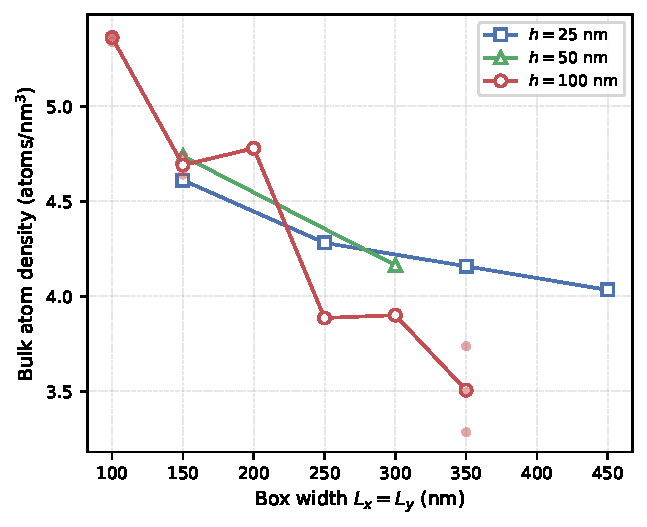
\includegraphics[width=0.7\linewidth]{boxconv_density_vs_L}
  \caption{%
    Bulk atom density falls monotonically with box width at every film
    height tested, with no sign of a plateau at the box size used in the
    main study -- direct visual evidence for the finite-size limitation
    discussed in Section~\ref{ssec:limits}.
    Bulk atom density versus box width $L$ for all trusted runs in the
    finite-size convergence campaign, grouped by film height $h$
    ($\dang = 85^{\circ}$, pitch $= 150$~nm fixed throughout).
    Lines connect the mean density at each $L$; small dots at
    $h=100$~nm, $L=350$~nm show the individual seed-replicate values
    behind that mean.
  }
  \label{fig:boxconv}
\end{figure}

A box-size sweep ($L_x=L_y \in \{75,100,125,150\}$~nm at $\dang=85^{\circ}$,
pitch $=\SI{150}{nm}$ fixed) shows the mean atom areal density decreases
monotonically and substantially with box size (by $\approx 29\%$ from
$\SI{75}{nm}$ to $\SI{150}{nm}$), with no sign of a plateau by
$L=\SI{150}{nm}$ (Figure~\ref{fig:boxconv}). The $\SI{100}{nm}$ box used throughout the main study is
therefore \emph{not} at a converged, asymptotic value; the true large-box
limit is likely lower still. Separately, a box size exactly equal to the
pitch ($L=\SI{150}{nm}=$~pitch) introduces an additional, sharper
commensurability artefact (erratic, non-physical atom counts at low
$\dang$) distinct from the smooth finite-size trend -- box sizes equal to
(or simple multiples/fractions of) the pitch should be avoided in future
campaigns. Attempts to extend the sweep beyond $L=\SI{150}{nm}$ in this
first pass were constrained by the simulator's GPU memory management
rather than by physics.

A subsequent height-matched scan ($h=\SI{25}{nm}$, $L\in\{150,250,350,450\}$~nm)
confirmed the density keeps decreasing with no plateau, and showed that a
single-variable finite-size scaling collapse (density as a function of
$L/(h\tan\dang)$ alone) does not hold across different heights -- at least
two physical length scales (the finite-size shadow length and a
substrate-proximity transient) govern the box-size dependence, so the
large-box asymptote and a corrected scaling ansatz remain open questions
for future work. Cross-checking the $L=100$ vs $\SI{150}{nm}$ density
change at three angles ($\dang=75,85,89^{\circ}$) shows this bias is
\emph{not} angle-independent ($-32\%,-21\%,-20\%$ respectively): the
angular trend reported in the main text, while qualitatively consistent
with the literature comparisons discussed there, should be read as
possibly compressed or shifted in magnitude by an angle-dependent
finite-size effect that a fixed box size cannot separate from the true
physics.

A subsequent degeneracy-breaking campaign (three additional targeted runs:
$h=\SI{50}{nm}$ at $L=150$ and $\SI{300}{nm}$, and a second seed at
$h=\SI{100}{nm}$, $L=\SI{350}{nm}$) extended the height-matched scan above
to a third distinct film height and provided the first genuine
seed-replicate at large $L$. Fitting a multiplicative
shadow-decay$\times$substrate-transient model, $\rho(L,h) = \rho_\infty -
A\,(1-e^{-h/\tau})\,e^{-L/\lambda}$, with a heteroscedastic weighting
exponent $p$ swept over $\{0.5,0.75,1.0\}$ (rather than fixed, since $p$ is
a closure-model choice, not an estimable constant, at this data volume)
gives $\rho_\infty$ point estimates of $4.28$, $4.19$, and $4.03$
atoms/nm$^3$ respectively, with $95\%$ bootstrap confidence intervals that
overlap across all three $p$; the substrate-transient amplitude $A$ is
consistently unresolvable (pinned near zero for every $p$), confirming
that only $\rho_\infty$, not the transient term, is currently informative
from this data. Independently, a real-space pair-correlation length
$\xi(L)$ measured directly from atom positions (not from the voxelised
pipeline) is still increasing at $L=\SI{350}{nm}$ across the $h=25$, $50$,
and $\SI{100}{nm}$ series alike -- consistent with, and independent
evidence for, the absence of a finite-size plateau reported above. One run
in the original height-matched scan ($h=\SI{25}{nm}$, $L=\SI{250}{nm}$) had
originally failed an automated column-tilt validation gate; this was
root-caused to a validator threshold that incorrectly ran a straight-column
tilt regression on a genuinely (if only briefly) rotating deposit, producing
a spurious result -- the underlying atom data for that run is sound and it
is retained in the trusted dataset once the validator was corrected.

\textbf{A resolved but consequential finding:} a third seed at
$L=\SI{350}{nm}$ was run specifically to place the large-$L$ variance
estimate on the same statistical footing ($n=3$) as the $L=100$ anchor.
With this third replicate, the empirical relative seed-to-seed variance in
areal density is confirmed to \emph{grow}, not shrink, with box size:
$L=100$: $0.32\%$ ($n=3$); $L=150$: $1.09\%$ ($n=2$); $L=350$: $5.28\%$
($n=3$) -- an approximately $16\times$ increase in relative scatter from
the smallest to the largest box, on equal ($n=3$) statistical footing at
the two endpoints, not a two-point artefact. This is the opposite trend
from the shrinking variance assumed by every $p$ tested above (all
presuppose $N_{\mathrm{col}}\!\sim\!L^2$ independent columns
self-averaging down the noise), and it is large enough to matter: refitting
with a growing-variance weight $\sigma(L)\propto (L/L_{\mathrm{ref}})^{q}$,
with $q$ estimated directly from these three anchors ($q\approx2.18$) or
swept over $\{1.0,2.0,2.5\}$, gives $\rho_\infty \approx 4.9$--$5.2$
atoms/nm$^3$ -- materially higher than, and non-overlapping with, the
$4.0$--$4.3$ atoms/nm$^3$ range obtained under the originally-assumed
shrinking-variance closure. We therefore report $\rho_\infty$ as
$4.9$--$5.2$ atoms/nm$^3$ under the empirically-supported growing-variance
weighting, and flag the shrinking-variance value as based on a
now-falsified assumption about how simulation noise scales with box size,
retained here only for transparency about how much a single modelling
choice can move this number. We do not currently have a first-principles
explanation for why relative fluctuations grow with $L$ in this simulator;
the most plausible hypothesis links it to the non-saturating $\xi(L)$
reported above (a growing transverse correlation length implies the
effective number of statistically-independent columns grows more slowly
than $L^2$, which would suppress rather than enhance self-averaging at
large $L$), but confirming this mechanism -- as opposed to merely being
consistent with it -- is future work. Practically, this means finite-size
extrapolation in this system is noise-limited by a growing, not shrinking,
per-box uncertainty at large $L$, so additional seeds at large $L$ (rather
than additional, more expensive large-$L$ single runs) are the more
statistically efficient way to tighten $\rho_\infty$ further.

Two claim tiers follow from the box-size result above and should not be
conflated. \emph{Quantitative} absolute values reported anywhere in the
main text -- the void-fraction endpoints ($94.2\%$, $99.4\%$), the PCA
variance-explained figure, the \textsc{CorrNIF} $R^2$ values, and the
Maxwell-Garnett birefringence magnitudes -- are all computed at the
$\SI{100}{nm}$-box convention and are provisional: given the density
shifts documented above, their numerical values would change at a larger,
still-unconverged box size, and none should be read as an asymptotic
result. \emph{Qualitative}, monotonic angle-orderings (void fraction
rising with $\dang$; birefringence falling with $\dang$ in the literature
comparison of Section~\ref{ssec:nif_optical}) are the category of claim
least exposed to this limitation in principle, but at present this project
can only offer partial, not conclusive, support for that expectation: a
box-size cross-check exists at just three angles ($\dang = 75, 85,
89^{\circ}$), it is itself confounded by a simultaneously reduced
active-window parameter, and within it the openness proxy shifted upward
by a small, similarly-sized amount at all three angles (consistent with,
but not proof of, order-preservation) while a different descriptor
computed on the same box-size campaign, $\beta_{\mathrm{sim}}(\dang)$, was
found to be non-monotonic and its box-size dependence remains unresolved.
We therefore do not assert that the monotonic orderings reported here are
established to be box-size-robust; they should also be treated as
provisional pending an angle-resolved convergence study, and are offered
as the paper's best-supported trend-level claims rather than as
finite-size-independent results.

\section{Coordination-shell cutoff factor: geometric derivation}
\label{app:shellcutoff}

This appendix derives the valid range for the coordination-shell cutoff
factor $k$ used by the diffuse re-emission ablation of
Section~\ref{ssec:limits}, where the cutoff radius for counting a
neighbouring atom as belonging to the first coordination shell is
$R(k) = k \times d_{\mathrm{col}}$, with $d_{\mathrm{col}}$ the model's
hard-sphere collision diameter. This model uses $k=1.15$.

For a face-centred-cubic (FCC) lattice with conventional cubic cell edge
$a$, the nearest-neighbour (NN) and next-nearest-neighbour (NNN)
distances are
\begin{align}
  d_{\mathrm{NN}}  &= a/\sqrt{2}, \label{eq:app_dnn}\\
  d_{\mathrm{NNN}} &= a. \label{eq:app_dnnn}
\end{align}
For Cu, $a=\SI{3.615}{\angstrom}$ \citep{straumanis1969} gives
$d_{\mathrm{NN}}=\SI{0.2556}{nm}$, $d_{\mathrm{NNN}}=\SI{0.3615}{nm}$, in
agreement (within $0.16\%$) with this model's independently-derived
collision diameter $d_{\mathrm{col}}=2\times\SI{0.128}{nm}=\SI{0.256}{nm}$
(Cordero covalent radius \citep{cordero2008}) -- both are estimates of
the same physical Cu--Cu contact length scale from independent routes,
so their agreement is a consistency check on the model's basic geometry,
not a new claim.

A cutoff factor $k$ isolates the true first shell -- counting every atom
in physical contact, $R(k)\ge d_{\mathrm{NN}}$, while excluding the
second shell, $R(k) < d_{\mathrm{NNN}}$ -- exactly when
\begin{equation}
  1 \le k < \frac{d_{\mathrm{NNN}}}{d_{\mathrm{NN}}} = \sqrt{2} \approx 1.41421.
  \label{eq:app_kwindow}
\end{equation}
This half-open interval $k\in[1,\sqrt{2})$ follows from FCC geometry
alone (Eqs.~\ref{eq:app_dnn}--\ref{eq:app_dnnn}); it does not depend on
which value inside it is chosen. The value used here, $k=1.15$, sits at
\begin{equation}
  f = \frac{k-1}{\sqrt{2}-1} \approx 0.362,
  \label{eq:app_kfrac}
\end{equation}
i.e.\ $36.2\%$ of the way from the NN boundary to the NNN boundary, with
margins of $\SI{0.038}{nm}$ above the NN boundary and $\SI{0.068}{nm}$
below the NNN boundary -- comfortably inside the valid window on both
sides, not adjacent to either boundary. Both margins exceed the scale of
typical thermal/structural broadening expected in this model's
disordered, non-rigid-lattice packing (\S\ref{ssec:limits}), which is
the practical reason an interior value is preferable to one sitting
exactly at either boundary.

This derivation establishes the \emph{interval} $k\in[1,\sqrt{2})$ as
geometrically required; it does not establish that $k=1.15$
specifically, as opposed to another interior value, is uniquely forced
by the crystallography. No record of the original reasoning behind the
specific value $1.15$ exists in this project's development history, and
an exhaustive literature search and a full-text search of $1{,}695$ PDF
documents held locally by this project found no external source
proposing this specific value for an FCC-metal first-shell cutoff.
$k=1.15$ is therefore reported here as a documented, geometrically
justified modelling convention selected from within a rigorously
derived valid range, not as a value independently confirmed by an
external source.

\end{document}
